\pagebreak

\begin{quote}
\begin{flushright}
\textit{La guêpe et l'orchidée font rhizome, en tant que hétérogènes}\end{flushright}

\begin{flushright}
\text{Deleuze and Guattari}, \textit{Plateau mille} \end{flushright}

\end{quote}

\begin{quote}
\begin{flushright}
\textit{Given the nature of all this new shit, you know, I-I-I-I... this could be a-a-a-a lot more, uh, uh, uh, uh, uh, uh, complex, I mean, it's not just, it might not be just such a simple... uh, you know?} \end{flushright}

\begin{flushright}
\text{Joel \& Ethan Coen}, \textit{The Big Lebowski } \text{(1997)} \end{flushright}
\end{quote}

\hypertarget{introduction}{%
\section{Introduction}\label{introduction}}

In Edmond Halley's \emph{Synopsis of the Astronomy of Comets} (1705),
Halley used Newton's model of gravitation to estimate the orbit of his
now eponymous comet. Halley conjectured that past observations of
``different'' comets, each appearing roughly 76 years after the
previous, were in fact the same object, and that the variability in the
comet's period was attributable to the variable gravitational influence
of Jupiter and Saturn. Halley's computations enabled him to predict his
comet's eventual return to Earth in 1758, and although he didn't live to
observe his prediction come true, his work helped provide the initial
validation of much of Newtonian mechanics.

The success of Halley's prediction also further fortified the methods of
Cartesian reductionism as the principal ideology in scientific
understanding. In physics, the problem solving strategy of starting with
the simplest case and gradually building toward a higher fidelity
representation of the system is so ubiquitous it is applied without even
mentioning that is what's happening. However, in ecology, this approach
often does not succeed because the properties of the systems we seek to
understand do not exist when we reduce a system down to its individual
parts. For example, consider the Lotka-Volterra model. Much like the
model of Newtonian gravity Halley applied to his comet, LV is written in
the language of ordinary-differential equations\footnote{The reality is
  computing the gravitational dynamics of more than two bodies of
  comparable mass is, much like ecological modeling, tough. Halley was
  able to work around the infamous n-body problem, but modern
  astrodynamicists use simulation models for many of the same reasons we
  advocate their use in ecology, coming up in the main text.}. Yet, LV
doesn't succeed predicting the true abundance of predator-and-prey
species in most systems with much accuracy, 76 years out or otherwise.
This is not to say the LV model is not interesting and worthy of study
in its own right--it is what Okubo (1972) calls a ``toy model''--an
intentional oversimplification that can illuminate the dynamics pf real
systems (clean sentence up). The characteristic feature of the LV model
are its boom-and-bust limit cycles, and this qualitative behavior is
observed in many systems. However, for the purposes of inference and
forecasting, there is at least enough influence on the abundance of each
species from the combined factors of environmental and demographic
stochasticity, trait-matching, spatial distributions, and so on, that LV
isn't suited for applications in conservation management.

Trophic interactions between pairs of species are the building blocks of
ecological communities, and yet the properties of communities cannot be
understood simply by generalizing LV to larger systems (May), as there
are latent processes structuring communities that are only apparent
outside the scope of any particular interaction between two species.
This is the essence of what make any system \emph{complex}.

There is no natural system that is not complex. The motion of matter is
subject to the ever-changing pairwise gravitational forces of all matter
in existence, and

Ecosystems are emergent phenomena, stochastic and variable at all
scales. In biology, we find that our attempts to reduce a systems down
to the level of atomic units does not necessarily succeed because at any
level of biological organization there is internal heterogeneity (Levins
and Lewontin). In community ecology, it seems that atomic level of
organization is naturally the individual of a given species. Yet,
adopting the Platonic form ``individual'' neglects the immense
variability in the processes that compose any given individual.
Certainly this abstraction would cause consternation from the behavioral
ecologists down the hall, to the cell biologists studying gene
expression, to the biochemists doing, uh, you know, biochemistry. This
is not to say that we should build ecological models starting from the
building blocks of particle physics to thoroughly encapsulate the
heterogeneity across the spectrum of levels of biological organization
(Levins 1992), but instead we must be cognizant of what our models treat
as internally homogeneous--a false premise in biological systems.

Bottom up vs.~top-down models--how does this relate to \(A\)?

\begin{quote}
A space capsule could not land on the moon without Newtonian
abstractions, nor could it land with them alone. The problem for science
is to understand the proper domain of explanation of each abstraction
rather than become its prisoner.

Lewontin and Levins (1978?)
\end{quote}

Simulation models have generally upended the methods of science across
all disciplines because they enable us to explore the ``proper domain of
explanation of each abstraction'' with more care, and often less
required expertise, than the tools of analytical math. We can directly
incorporate stochastic behavior into our models, and the modular nature
of software means any conceptual object used in a simulation model can
be represented in as much fidelity as the author chooses. One can
implement the LV model (without any in-depth knowledge of how to solve
differential equations, in fact) in 30 lines of code, or create the most
convoluted individual-based model imaginable--it then becomes within the
author's purview to define the ``proper domain of explanation of each
abstraction''.

Using simulation models, we contest, we can now explore the complex
processes that produce the astounding biodiversity we see on Earth in
far more detail, and with greater respect toward their complexity.
Further, these tools have potential as we attempt to understand the
dramatic influence humans have on our planet and the life to which it is
a unique home. Simulation models have long been used for forecasting and
inference in complex systems. One does not struggle to list fields where
simulation models are a ubiquitous tool of the trade--climate science,
meteorology, epidemiology, etc. Ecology has much to gain in adopting
these methods as regular.

There are certainly challenges in this domain--how do we find a bridge
between complex simulation models and data? How do we validate that
these simulation models `work', in that they accurately represent the
ecological process they are meant to model?---some potential answers
will be discussed further in the next section.

The primary goal of this prospectus is to outline the benefits and
future applications of simulation models in biodiversity science, both
for the purposes of answering ``purely'' scientific questions, but also
for forecasting and management in real ecological systems. Most studies
which incorporate simulation tend to fall into one of two categories:
the first being where the simulation model is used as a ``virtual
laboratory'' (@volker\_grimm\_ibm) to experiment with systems that do
not fit into the spatial/temporal scale that can be done in real life,
the second being for the application of a simulation model to a real
system. In the ``virtual laboratory'' case, the parameter values often
are meant to encapsulate the the entire spectrum of possible values, are
based in what the researcher (or reviewers) find interesting. In the
second case, parameter inference is vital in producing useful
predictions.

Here, we outline how simulation models can be used to make predictions
with real data. We then describe a process-based model of metacommunity
dynamics (based around @poisot\_2014 and @velland\_2010, that recent
ecology letters paper). We then detail how we'll implement this model as
software that is modular and can be used to answer questions in the
``virtual laboratory'' case, as well as to be fit for real systems. We
then conclude by outlining the structure/point of each dissertation
chapter.

The product at the end of the dissertation is this software package, and
the chapters are structured as an introduction and review, software
paper, and then chapters that utilize the software in varying
capacities: first as a `virtual laboratory' to answer niche
vs.~neutrality question. Then as a interface to local system
data--forecasting connectivity in Montreal. Finally as larger-scale
inference, when we consider climate model projections

\hypertarget{literature-overview}{%
\section{Literature Overview}\label{literature-overview}}

biodiversity has many dimensions, here we focus on community. rhizomatic
field of study, no de facto entrance.

get at the fundamental questions again and that;s why you are reviewing
these fields.

\hypertarget{models-and-data}{%
\subsection{Models and Data}\label{models-and-data}}

I would classify the vast majority of time I spend ``working'' (under
the categories of) building, interpreting, thinking, reading, writing,
and talking about models. So what are these models? For a model to be
falsifiable, it must map observable input conditions \(x\) to observable
output conditions \(y\) as a function of both \(x\) and model parameters
\(\theta\) which typically are scalar coefficients used in the
definition of the mapping \(y = f(\hat{x}, \theta)\).

If \(\hat{y} \approx y\), we say our model \(f\) is ``good'', and we
Google ``Nature submission instructions''. If not, we say our model is
bad and try something else. Model selection has deep and rich history,
starting somewhere near ``Occam's Razor'' and ending far outside the
scope of this document. For our purposes, it suffices to understand that
there exist several model selection criteria that enable us to determine
which of a set of competing explanatory models, \(\{f_1, f_2, \dots\}\)
provides the highest fidelity explanation of our data. Model validation
for complex systems is a

Many of the more popular methods (AIC, BIC, MDL, k-fold crossvalidation)
follow the hueristic that models should maximize the ratio of the
information they provide in predictive power to the amount of
information they contain in their definition.

What separates science from philosophy? For most of recorded human
history, science and philosophy were not separate disciplines, and most
languages didn't have words to distinguish a scientist from a
philosopher. Both provide explanations of the world in the form of
models, and both

\begin{quote}
In fact, the sciences, arts, and philosophies are all equally creators.
. . Concepts do not wait for us ready-made, like celestial bodies. There
is no heaven for concepts. They must be invented, fabricated, or rather
created, and would be nothing without the signature of those who create
them. (Deleuze \& Guattari 1991)
\end{quote}

I would contest science restricts itself to models that allow some
interface between the conceptual models we make and that which is
observable about the world, such that they can be compared with
so-called `ground truth'---all scientific models must define some set of
conceptual objects \(A \in \text{Universe}\).

To make a comparison between a model and ``ground truth'', there must be
some way to observe and measure the concepts \(A\). More formally, there
must be some observation mapping \(O: A \to \mathbb{R}^{d_1}\), where
\(d_1\) is the dimensionality of our measuremennt. And so scientific
models inevitably create a mapping between observable states of the
concepts as we define them, and quantitative predicted outcomes,
\(f : O(A) \to \mathbb{R}^{d_2}\). (Generally, \(d_2 << d_1\), otherwise
we've just found a new way of shuffling around the same information in
the data.)

In Halley's model
\(A = \{\text{Sun}, \text{Jupiter}, \text{Saturn}, \text{Earth}, \text{Comet} \}\),
and \(O(A) = \{\text{mass}, \text{position}, \text{momentum}\}\).

And so those who are interested in (building, designing, using, etc.)
models face the task of defining \(f\) in such a way that it (hopefully)
makes accurate predictions.

We can broadly split models into two types: process models and
statistical models (@mcelreath). Other types of statistical models
(typically those that fall under the ambiguous banner ``machine
learning'') do not define \(f\) with much regard towards the actual
concepts in \(A\) at all, but instead are cleverly designed algorithms
which can accurately map input conditions to output conditions in some
cases. Models do many different things: hypothesis testing, inference,
parameter estimation, forecasting,etc. Often, when we do science, models
are only a bridge between the data we collect and actual hypotheses. See
the figure below from @mcelreath.

\begin{figure}
\centering
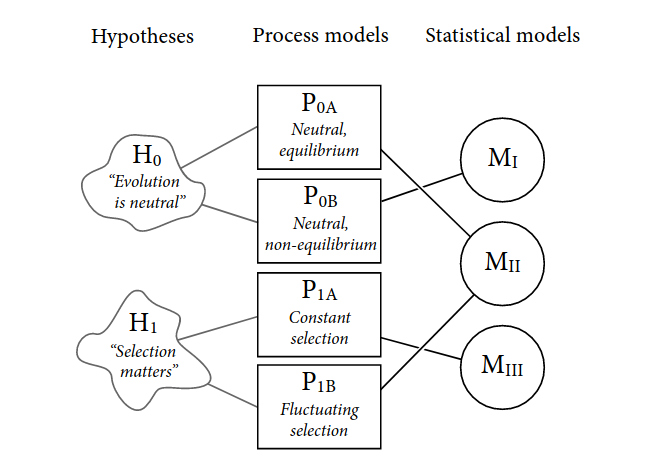
\includegraphics{/home/michael/prospectus/figures/mcelreath.png}
\caption{From McElreath 2019--the relationship between hypotheses,
process models, and statistical models represented as a network.
Original caption: \emph{Relations among hypotheses (left), detailed
process models (middle), and statistical models (right), illustrated by
the example of ``neu- tral'' models of evolution. Hypotheses (H) are
typically vague, and so cor- respond to more than one process model (P).
Statistical evaluations of hy- potheses rarely address process models
directly. Instead, they rely upon statistical models (M), all of which
reflect only some aspects of the process models. As a result, relations
are multiple in both directions: Hypotheses do not imply unique models,
and models do not imply unique hypotheses. This fact greatly complicates
statistical inference.}}
\end{figure}

There are no natural isomorphisms from hypotheses to statistical
models---conflicting hypotheses can be consistent with a single result
of a statistical model if the statistical model produces the same
outcomes under processes that correspond to conflicting hypotheses.

Nearly all statistical models function by reducing the dimensionality of
our data. This is often done out of sheer necessity, either for
degrees-of-freedom or sanity--however an unfortunate byproduct of some
summary statistics is that they produce the same results under differing
process models. To use the example from Figure 1, models for inferring
selection historically rely on summary statistics like \(F_{ST}\), often
summarized across multiple loci, in order to ``test'' the observed value
of \(F_{ST}\) against some expectation, like migration-drift balance, to
determine if there is evidence of selection.

Process models use conceptual objects \(A\) that (at least with perfect
information) could be measured---dispersal, traits, environmental
conditions, etc. Summary statistics are usually pure abstractions that
may/may not correspond to anything in the real world.

Purely statistical models are certainly not without value. However, for
the purposes of inference and forecasting in biodiversity science, and
complex systems in general, the increasing availability of computing
power to simulate complex process models at large scales have enabled
the gap between process models and statistical models to shrink in
recent years.

In order to understand why ABC has significant potential in ecology, it
is best to start by asking: what is it that makes applying statistical
models to data so much easier than process models? The problem begins
with the difficulty of estimating the value of parameters in a process
model from real data. All models have parameters \(\theta\)---some
latent variables that cannot feasibly be measured, i.e.~all parameters
are conceptual objects outside of \(g(A)\).

As an example, consider fitting a species-distribution model (SDM),
\(y = f(x, \theta)\), where \(x\) is an environmental variable measured
across space, and \(y\) is the predicted probability of a given species
being present. To fit this model y = \(f(x, \theta)\), we need some
observed instances of both environmental conditions \(\hat{x}\) and
species occupancy \(\hat{y}\) in order to estimate \(\theta\). There are
seemingly unending methods of estimating \(\theta\) using a variety of
methods in both frequentist and Bayesian worlds, yet what the vast
majority of these methods have in common is that they estimate
\(\theta\) by using a likelihood function,
\(\mathbb{L}(\hat{x} | \theta)\), which is defined as the probability of
observing some data point \(\hat{x}\) given a model definition \(f\) and
some parameter values \(\theta\).

In a frequentist world, the likelihood function is a ubiquitous tool for
parameter inference. Most off-the-shelf statistical `tests',
e.g.~\texttt{model\ =\ lm(y\ \textasciitilde{}\ a*x\ +\ b)}, are simply
a repackaged likelihood function that can be used to estimate parameters
via maximum likelihood or any other frequentist estimation method.
Similarly, in a Bayesian world, the likelihood function is essential in
the application of Bayes' theorem to inference,

\[ P(\theta | \hat{x}) = \frac{P(\hat{x} | \theta)  P(\theta)}{P(\hat{x})} = \frac{\mathbb{L}(\hat{x}, \theta)  P(\theta)}{\int_\Theta \mathbb{L}(\hat{x} | \theta) P(\theta) d\theta}\]

If our model \(f\) is simple, we can write our likelihood down
analytically, e.g.~if we describe a naive SDM where the probability of
occurrence at a location in space \(\vec{L}\) is given by the difference
between the ``mean'' trait value of a species, \(T\), and the some
environmental condition \(E(\vec{L})\) related to the trait in
question\footnote{Of course, capturing the capacity for a species to
  persist using a single dimension is, to say the least, unlikely. The
  oversimplification here is in service of defining the most simple
  model possible.}, we can define a model \(f\) that says the
probability of occurrence at \(\vec{L}\) is a Gaussian evaluated at
\(E(\vec{L}) - T\), and induces a single parameter,
\(\theta = \{ \sigma \}\).

Because our model is defined with an analytically tractable
distribution, we can write down our likelihood
\(\mathbb{L}(x | \theta)\) fairly easily:
\[\mathbb{L}(\text{Species present at} \ \vec{L} \ |\  \sigma) = \frac{1}{\sigma \sqrt{2\pi}} \exp \Big( \frac{-(T-E(\vec{L}))^2}{2\sigma^2} \Big)\]

The ability to write our likelihood down in simple analytic terms means
that value of \(\mathbb{L}\) is straightforward to compute for any
values of \(T, E(\vec{L}),\) or \(\sigma\), and then we are free to
apply any number of parameter inference methods to estimate \(\sigma\) .
Once we estimate \(\sigma\), we can estimate the probability of
occurrence at any point in space \(L\) by simply evaluating
\(\mathbb{L}(\text{Species present} | E(L) , T, \sigma)\) at that
location, at which point we have a fully-fledged SDM.

What then, if we want to describe a model \(f\) where the probability of
occurrence is driven by both neutral changes in the spatial
distributions of each species, environmental stochasticity, variability
in species' traits in space and time, and so forth? One can imagine
constructing a monstrous likelihood function, compiled of distributions
stack on top of each other forever. But if one wants to introduce
covariance into these distributions, the appropriate tools for model
fitting and validation quickly begins to require statistical expertise
that is beyond what is reasonable for any non-practitioner of the field
to know, especially for ecologists who are devoted to the management of
a particular system and are also asked to have in-depth knowledge of its
natural history, etc. Thankfully, we have software like STAN which makes
application of more complex models like this to be written and applied
quickly, however such models still inevitably rely on assumptions about
processes that have been abstracted away from the mechanism producing
the data, and instead toward a statistical representation of a process
that is subject to the pitfalls presented in Figure 1.

The gap between statistical and process models has long been caused by
the intractability of the likelihood function for complex stochastic
processes. However, modern computational power enables us to simulate
many replicates of stochastic simulation models, we can treat the
distribution of simulation model outcomes as approaching the likelihood
function as the number of replicates increases\footnote{There are
  several caveats here, all outside the scope of this document}. Methods
for bridging the gap between empirical data and complex simulation
models have go under many names--Bayesian nonparametric
methods\footnote{This term can be confusing, as ``nonparametric'' models
  in fact have a parameter space of infinite-dimension
  @orbanz\_bayesian\_2015}, likelihood-free inference--but in ecology
and evolutionary biology, these methods tend to be classified under the
term Approximate Bayesian Computation (ABC), which was introduced by
Beaumont 2002 {[}@beaumont{]} for applications in evolutionary
genetics---conveniently, with respect to the evolutionary genetics
example from Figure 1. ABC methods in evolutionary genetics tend to
begin with a researcher implementing a simulation model whereby genomes,
individuals, and populations are represented at any level of detail
imaginable.

One can then use ABC methods to infer model parameters, and to use model
selection criteria to determine which mechanistic process is more likely
to have produced a set of data.

There is still a reliance on summary statistics, but if summary
statistics are not differentiable even when the generative process is
different, that itself is interesting, and, in general, simulation
models are excellent testing grounds for the biases of summary
statistics (see Jost's D vs Fst etc).

Remaining questions:

\begin{itemize}
\item
  prior selection
\item
  model validation
\item
  simulation time -- regression model to estimate likelihood
\item
\end{itemize}

\hypertarget{community-structure}{%
\subsection{Community Structure}\label{community-structure}}

The search for generality among ecological communities long flummoxed
early ecologists, culminating in the aphorism that community ecology is
``a mess'' (citation).

homage to santa rosalia, biodiversity questions via community structure

Early theoretical work on community structure begins with the
Diversity-Stability ``Paradox'', largely attributed to May's \emph{Will
a Large Complex System be Stable} (@cite) and \emph{Stability and
Complex is Model Ecosystems} (@cite). May's work considered both a
linear system, \(\dot{x} = A\vec{x}\), and a generalized Lotka-Volterra
system, \(\dot{x} = \vec{x} \odot (A \vec{x} + \vec{g})\), where
\(\vec{x}\) is a vector of abundances, \(\vec{g}\) is a vector of change
in abundance absent any consumption and \(A_{ij}\) between any species
\(i\) and \(j\) is the interaction strength\footnote{itself a term
  fraught with ambiguity} .

May's computations showed that as the number of species \(N_s\) in the
randomly generated food-web \(A\) increased, the probability that the
system persists approaches \(0\). There is where the so-called `paradox'
lies--we observe food-webs in nature that are interwoven between far
more species than we would expect under May's neutral model, and so
naturally the study of complexity in food webs turned to both
understanding the processes that structure food webs such that they can
persist, and developing methods to infer the structure of ecological
networks.

What is `stable'? Fixed-point stability in a deterministic system. One
can compute the stability of a fixed-point by checking if the
eigenvalues of the Jacobian around any fixed point. For both of these
model, the Jacobian around a fixed point is always the adjacency matrix,
and so without computing any Jacobians we can simply check if
\(\{ \text{Re}(\lambda) < 0 \} \ \ \forall\lambda\) to determine if the
system has a fixed-point attractor. This is a method of computing
Lyapunov-stability of a fixed point in a system, and was tractable for
the computers of the time.

May's used a generative model of community structure where all terms
\[A_{ij} \sim Bernoulli(p)\]. This is the same as the graph generator
\(G(n,p)\), (Erdos).

Both in network science and ecology, generative models of network
structure have turned to embedding the verticies in a latent space from
which one follows a set of rules to determine which edges \(A_{ij}\)
exist. In ecology, the latent-space is typically a proxy for
trophic-level or allometric scaling, beginning with the Cascase model
(cite), drawing much more attention with the Niche model
(@williams\_martinez), and culminating in a generalized
multi-dimensional niche model with a likelihood function that can be
used to estimate latent parameters from empirical food webs (allesina).

In parallel, network science has developed its own set of generative
models for network structure which have several natural applications in
food web ecology. Stochastic-Block-Models (SBMs) have seen extensive use
for modular and nested network structures outside of ecology. There is a
trade-off between good fit and mechanisms in an SBM--it doesn't tell you
anything about the process making the data, it just learns how the
network its structured in such a way that it can generate structurally
similar networks.

One of the most powerful tools for problem-solving in mathematics is
paying attention to what is \emph{invariant} about a system, meaning
that which does not change in the system, even as we adjust its
parameters (Polya citation?). Ecosystems vary in seemingly dimensionless
ways. Yet, we can still find an invariant in ecology---the amount of
energy per unit area on the planet is a measurable value, and insofar as
we have any undisputed ``laws'' in science, one that is commonly
accepted is that energy has to go somewhere.

The application of thermodynamics to trophic communities led to a
renaissance(?) in our understanding of trophic community structure. We
directly had measurable things we could test against a model's
expectation, like allometric scaling (cite), metabolic use (cite), and
energy-efficiency in trophic interactions (cite). This enabled us to
make more sophisticated predictions about community structure in
empirical systems (stouffer paper, trophic theory islandbiogeo), and to
further develop generative models of ecological networks that fit
empirical food-webs.

It's true, the word `bioenergetic' does sound like I'm about to try to
sell you a collection of conveniently-priced crystals that will keep the
bears away. However, it is fewer syllables than any of its potential
synonyms, so I'm hoping we'll just be able to meet in the middle on this
one.

through poisot lab, a software package to simulate innes model with
diffeq solver

\begin{itemize}
\tightlist
\item
  real ecosystems are not governed by deterministic forces
\item
  stochasticity in interactions, for a variety of reasons
\end{itemize}

\hypertarget{spatial-ecology}{%
\subsection{Spatial Ecology}\label{spatial-ecology}}

Spatial ecology as it exists today would be radically different if not
for @macarthur\_and\_wilson. The Theory of Island Biogeography (TIBG) is
a foundation for both modern spatial and community ecology. TIBG
provides a mechanistic explanation for the species-area relationship,
one of the most well-established ``laws'' in ecology.

The theoretical construction of space used by
@macarthur\_and\_wilson---a set of internally homogeneous `islands',
each variable in size and surrounded by inhospitable water/matrix, each
either occupied or unoccupied by a particular species---has had deep
impacts on many modern methods used to infer ecological patterns across
space. Metapopulation theory, coined by @levins\_metapop, describes a
system of discrete habitat patches, all either occupied/unoccupied.
Modern occupancy models are rooted in this view of space: discrete
observations at spatial coordinates, with environmental covariates.

internally homogeneous islands, each a variable distance from the
mainland with a fixed `area'\footnote{area here corresponds to resource
  availability, and has to spatial significance in the model} and
distance from the mainland\footnote{a never-ending source of all species
  in the metaweb}

\begin{itemize}
\tightlist
\item
  every species has the same probability of colonization/extinction
\item
  the species richness at equilibrium as a function of the area
  replicates the species-area relationship
\item
  its a process model, which is good--however power-laws are ubiquitous
  patterns that occur as an outcome due to many different mechanistic
  processes (find the citation for this, i think its a Clauset paper)
\end{itemize}

However, a tension counter to discrete space runs throughout modern
spatial ecology. The availability of remote-sensing technology has
enabled the availability of `continuous' ecological data in the form of
rasters. As satellites designed for Earth Science orbit the Earth, they
bounce electromagnetic signals off the surface of our planet, and record
the spectral signature they receive reflected back at them. The
reflective signature of Earth's terrain can then be used to estimate
various properties about its surface---land cover, hydrology and
topography, abundance of abiotic resources like nitrogen and phosphorus,
and so on. The properties used by both different satellites and
different models vary widely in what they try to predict---from the
level of coarse land-cover categorizations to the presence of particular
species. Further, there is considerable variability in the spatial and
temporal scale at which data is collected.

From this, we can apply the metapopulation data--occupancy at points,
with environmental data at points, to produce rasters that estimate
species occupancy based on environmental data. These species
distribution models: max ent, bioclim. what is the strength of
environmental effects?

There is a difference in scale in what this type of data it provides,
what time period it covers, and what spatial resolution it has. This
``resolution gap'' is pervasive in most of the large-scale data sets
ecologists try to use: species, etc.

\hypertarget{metacommunities}{%
\subsection{Metacommunities}\label{metacommunities}}

Leibold et al.~(@leibold\_metacommunity\_2004) introduced the
metacommunity framework a synthesis of community and spatial ecology.
They define four paradigms under which previous research on the
interplay of community and spatial ecology can be categorized: 1) the
Species-Sorting perspective, 2) the Patch-Dynamics perspective, 3) the
Mass-Effect Perspective, and 4) the neutral perspective.

Although understanding the effects of spatial processes on community
structure has been a crucial part of the discipline since its rapid
growth in the 1950s and 1960s (@macarthur, @hutchinson), this work only
considered space solely as a domain in which the environment varies, and
each species was considered a static object in space in time, which are
distributed according to selection on environmental variables. This
forms the theoretical basis for niche theory as a mechanism behind
community structure, or what Leibold et al.~call the Species-Sorting
perspective of metacommunity dynamics. The Patch-Dynamics perspective is
rooted in the TIBG from above--occupancy dynamics on discrete,
internally homogeneous patches/islands, diversity limited by dispersal
The Mass-Effect perspective shifts to systems where dispersal drives
patterns of demography, rather than occupancy dynamics--sources and
sinks etc. Finally, the Neutral perspective considers community dynamics
driven by random drift, i.e.~at scales where there is not enough
variability in either selection or dispersal to drive variation of
community structure in space, other than the variability inherent to
random processes.

The methods used in each of the domains of these paradigms often
differed drastically--however Velland 2010 (@velland) argues that within
each of these four perspectives we see the same four fundamental
processes driving dynamics, just in different amounts. Velland's four
processes are selection, dispersal, drift, and speciation--functionally
the same as the four fundamental processes in evolutionary genetics,
which similarly deals with shifting compositions of units of over space
and time, the difference being that evolutionary genetics deals with
alleles, not species.

thompson 2020 ecology letters papers

At what point in the space of relative contributions of each process do
we get the dynamics described by each of Leibold et al.'s paradigms?

Ecological networks and biodiversity

\begin{itemize}
\tightlist
\item
  Poisot 2014s
\end{itemize}

How does the structure of an ecological network affect the ecosystem
functioning, and how does functioning relate to the ability for an
ecosystem to provide services to humans?

\begin{itemize}
\tightlist
\item
  @hooper\_global\_2012
\item
  @loreau\_biodiversity\_2002
\item
  @gonzalez\_estimating\_2016
\item
  @mouquet\_extinction\_2011
\item
  @urban\_improving\_2016
\item
  @balvanera\_linking\_2014
\item
  @thompson\_loss\_2017
\end{itemize}

\hypertarget{a-metacommunity-model}{%
\section{A Metacommunity Model}\label{a-metacommunity-model}}

\hypertarget{what-can-we-measure}{%
\subsection{What can we measure?}\label{what-can-we-measure}}

As we've explored, it is essential for a model \(f\) to interface with
observable quantities \(O(A)\) of the conceptual objects \(A\) that
\(f\) is structured around. Much of what drives community dynamics in
space and time is unobservable--the evolutionary life histories of
organisms lie outside the temporal limits of our observation, as do the
ecological conditions of the more-than extremely recent past. Even what
we can directly observe--abundance/occupancy, traits, genomes, etc.--are
subject to the limitations of exhaustive field work, which can only be
done on relatively small spatial scales.

metacommunitiesEspecially in the realm of data aggregated across large
spatial scales, we have databases composed of occupancy/abundance data,
traits, and interactions (mangal paper). But there are often differences
in the resolution of this data---e.g.~taxonomic/phylogenetic resolution.
In terms of abiotic data, we are enabled by advances in remote sensing,
which enable us to collect, with variable but ever-improving spatial and
temporal resolution, environmental variables like temperature,
precipitation, as well as land-usage maps, and more recently,
topographical and hydrological models of the Earth's surface. From other
fields we also have well-developed predictive models of climatology,
hydrology, and land-use, which can serve as inputs into our predictive
ecological models.

Abstracting and modularity of a model. There are four pieces that have
to be represented.

Generative models?? Why do we need generative models--

four parts:

\begin{enumerate}
\def\labelenumi{\arabic{enumi}.}
\item
  Community Model: \(\{M, B, \frac{\partial B}{\partial t}\}\)

  The topology of the metaweb \(M\), and the way the biomass \(B\) flows
  through the metaweb, \(\frac{\partial B}{\partial t}\).
\item
  Spatial Model: \(\{\Phi, L, H\}\)

  we have some set of locations \(L\) in a spatial domain \(S\). Each
  location \(x\) is associated with a value of habitat suitability
  \(H_i(L)\) for each species \(i\), and a dispersal potential
  \(\Phi_i(x \to y)\), which is the instantaneous probability that a
  unit of biomass from species \(i\) moves from
  \(x \to y \quad \forall x,y \in S\).
\item
  Selection Model: \(\{ T, H\}\)

  how do the traits \(T_i(x,t)\) of a species \(i\) at a location \(x\)
  at time \(t\) change?
  \(\frac{\partial T_i(x,t)}{\partial t} = w (H_i(x,t), T_i(x,t))\)

  \begin{enumerate}
  \def\labelenumii{\arabic{enumii}.}
  \tightlist
  \item
    phylogenetic reading
  \end{enumerate}
\item
  Community Summary Model \(\{ C(\hat{B}) \}\)

  A summary statistic which maps from the observed state of biomass
  abundance (or occupancy) at some place and time to a number indicative
  of network properties. e.g.~Shannon-entropy as a measure of
  \(\alpha\)-diversity
\end{enumerate}

So now we have a set of conceptual objects,
\(A = \{B, L, M, T, \Phi, H, C, \frac{\partial B}{\partial t} \frac{\partial T}{\partial t}\}\)
in our model.

\begin{figure}
\centering
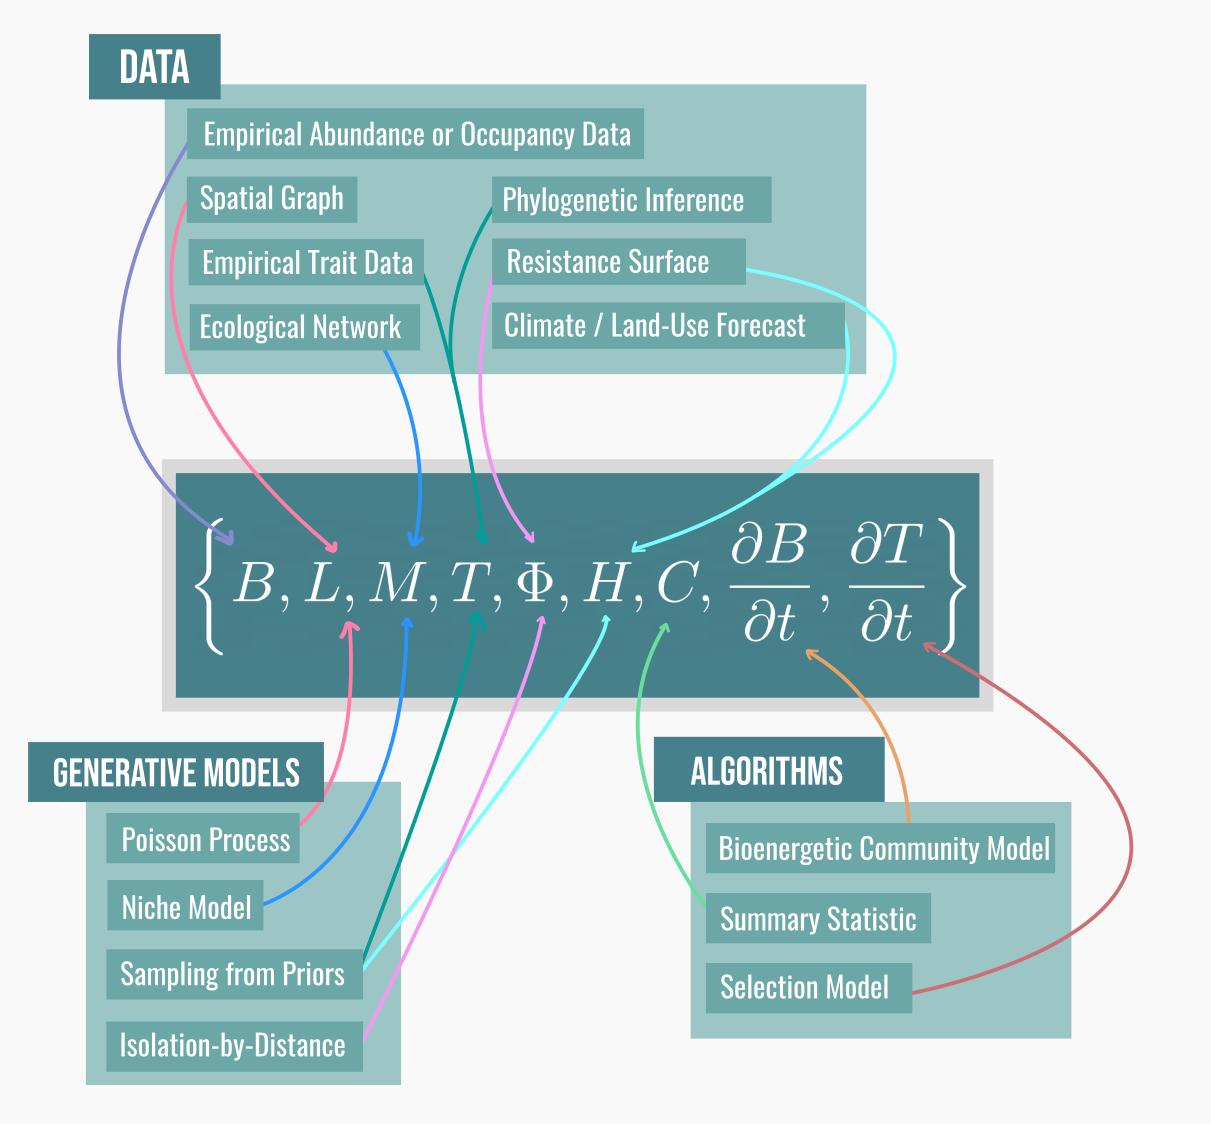
\includegraphics{/home/michael/prospectus/figures/inputs.png}
\caption{this is a caption}
\end{figure}

Software component--how does it interface with real data, and how does
it work as a `virtual lab'--

ABC figure here,info criteria figure here

\hypertarget{community-model}{%
\subsection{1. Community Model}\label{community-model}}

What is a community? Energy flow on a graph. How do we model energy flow
on a graph?

Two components, the topology of the metaweb, \(A\), and dynamics,
\(\frac{\partial B}{\partial t}\)

\hypertarget{a.-a-generative-model-of-food-web-topology}{%
\subsubsection{a. A Generative Model of Food-Web
Topology}\label{a.-a-generative-model-of-food-web-topology}}

Takes on parameters, \(\theta_T = \{\dots\}\), and produces a metaweb,
\(A = \begin{bmatrix} A_{ij} \end{bmatrix}\), where
\[A_{ij} = \begin{cases}1 \quad\quad& \text{if interaction is possible} \\ 0 & \text{otherwise}\end{cases}\]

\begin{itemize}
\tightlist
\item
  Niche Model, @williams\_simple\_2000

  \begin{itemize}
  \tightlist
  \item
    \(\theta_T\) :

    \begin{itemize}
    \tightlist
    \item
      number of species, \(N_s\)
    \item
      connectance, \(C\)
    \end{itemize}
  \item
    other parameters can represent structure, etc. allesina
  \end{itemize}
\end{itemize}

\hypertarget{b.-thermodynamic-consumer-resource-model-tcrm}{%
\subsubsection{b. Thermodynamic Consumer-Resource Model
(TCRM)}\label{b.-thermodynamic-consumer-resource-model-tcrm}}

Ecology has long struggled to find generality. There are
invariants/constraints in community ecology, so lets use them.

\begin{itemize}
\item
  Biomass distribution across species, \(\vec{B}(t)\).
\item
  Bioenergetic model \(\frac{\partial B}{\partial t}\), dominguez-garcia
  et al and history.
\item
  Species trait distributions

  \begin{itemize}
  \tightlist
  \item
    \(T_i(t, \vec{x})\).
  \end{itemize}
\item
  Interaction potential \[[ \Phi_{ij}  ] = f(\vec{T}, \vec{B})\]
\item
  thermodynamic consumer-resource model (tcrm)
  \[\frac{d\vec{B}_i}{dt} = r_i G_i B_i + \sum_{j \in \text{prey}} [e_{0j}F_{ij}] - \sum_{k \in \text{prod}} [B_k F_{ki}] - x_i B_i - d_i B_i\]

  \begin{itemize}
  \tightlist
  \item
    \(r_i\) : indicator for plants/primary production
    \[r_i = \begin{cases} 1 \quad\quad\quad &\text{if } i \text{ is a primary producer} \\ 0 &\text{otherwise}\end{cases}\]
  \item
    \(x_i\): metabolic demand for species \(i\)
    \[x_i = \begin{cases} 0.138m_i^{0.25} \quad\quad\quad & \text{if primary producer} \\ 0.314m_i^{0.25} & \text{else} \end{cases}\]
  \item
    \(d_i\): natural mortality rate \[d_i  = d_0 x_i \] with
    \(d_0 = 0.1\)
  \item
    \(e_{ij}\) : efficiency of energy conversion from \(i \to j\)
  \item
    \(G_i\): growth of primary producers
  \item
    \(F_{ij}\) : functional response \(i \to j\)
  \end{itemize}
\end{itemize}

\hypertarget{spatial-model}{%
\subsection{2. Spatial Model}\label{spatial-model}}

\begin{figure}
\centering
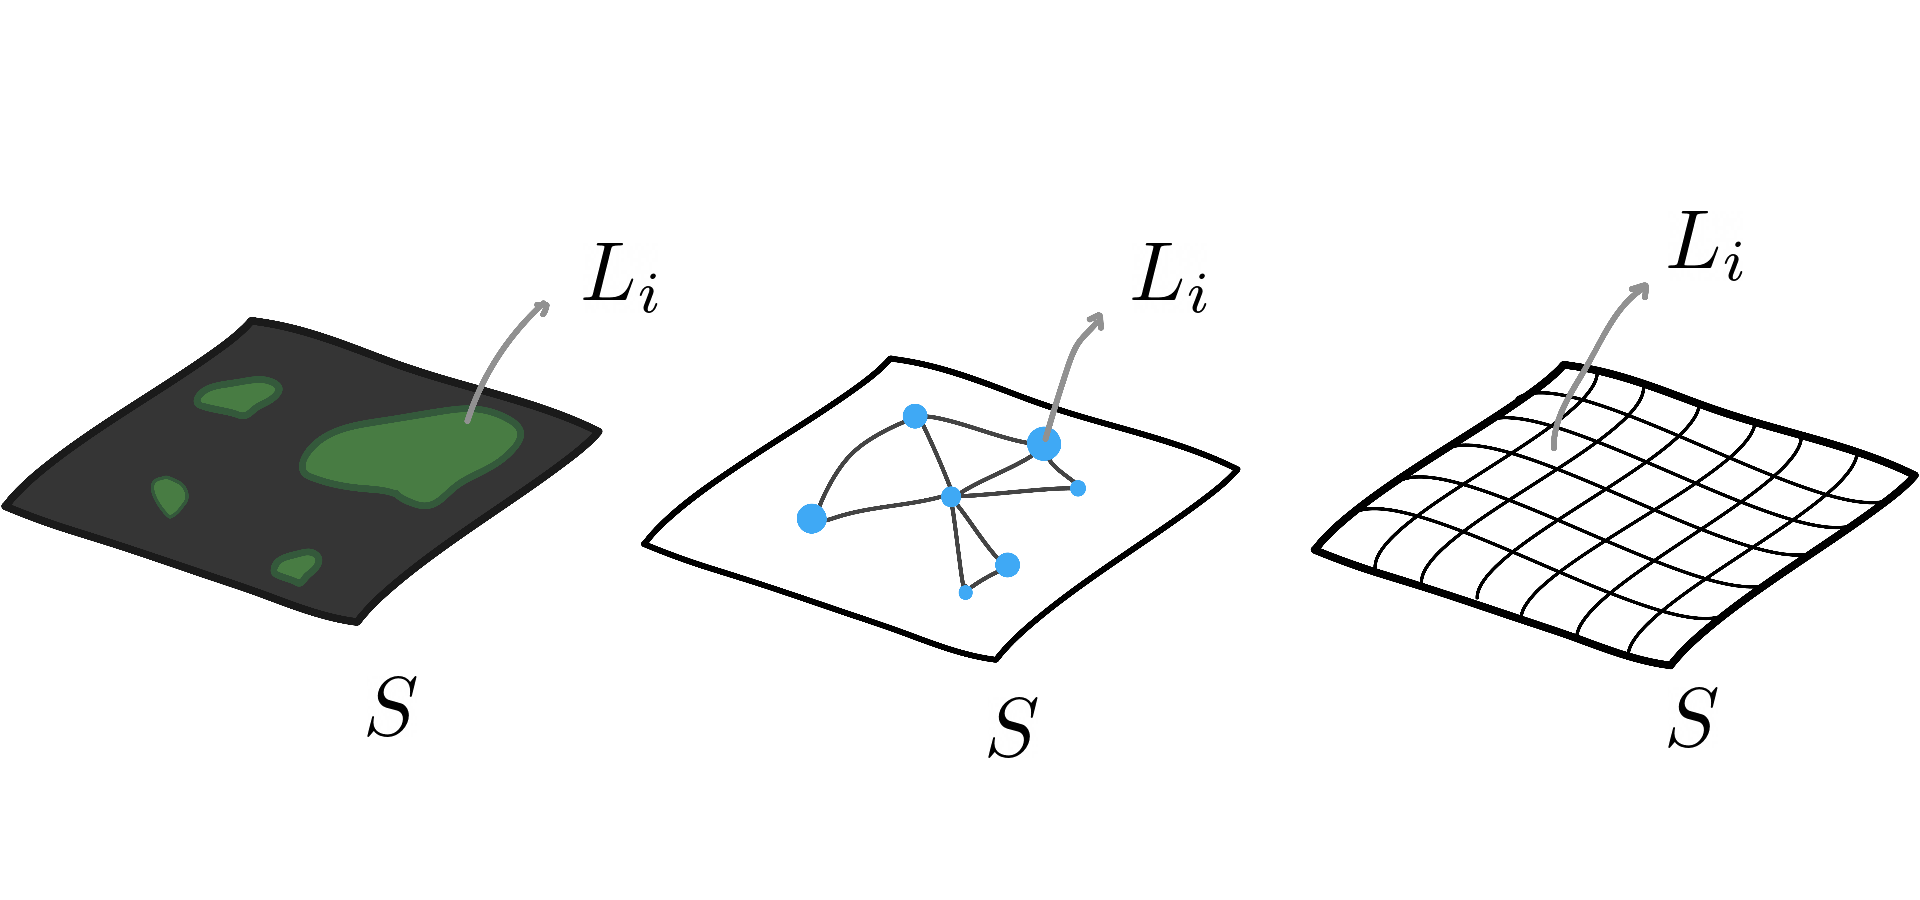
\includegraphics{/home/michael/prospectus/figures/different_spatial_models_w_labels.png}
\caption{this is a caption}
\end{figure}

\begin{figure}
\centering
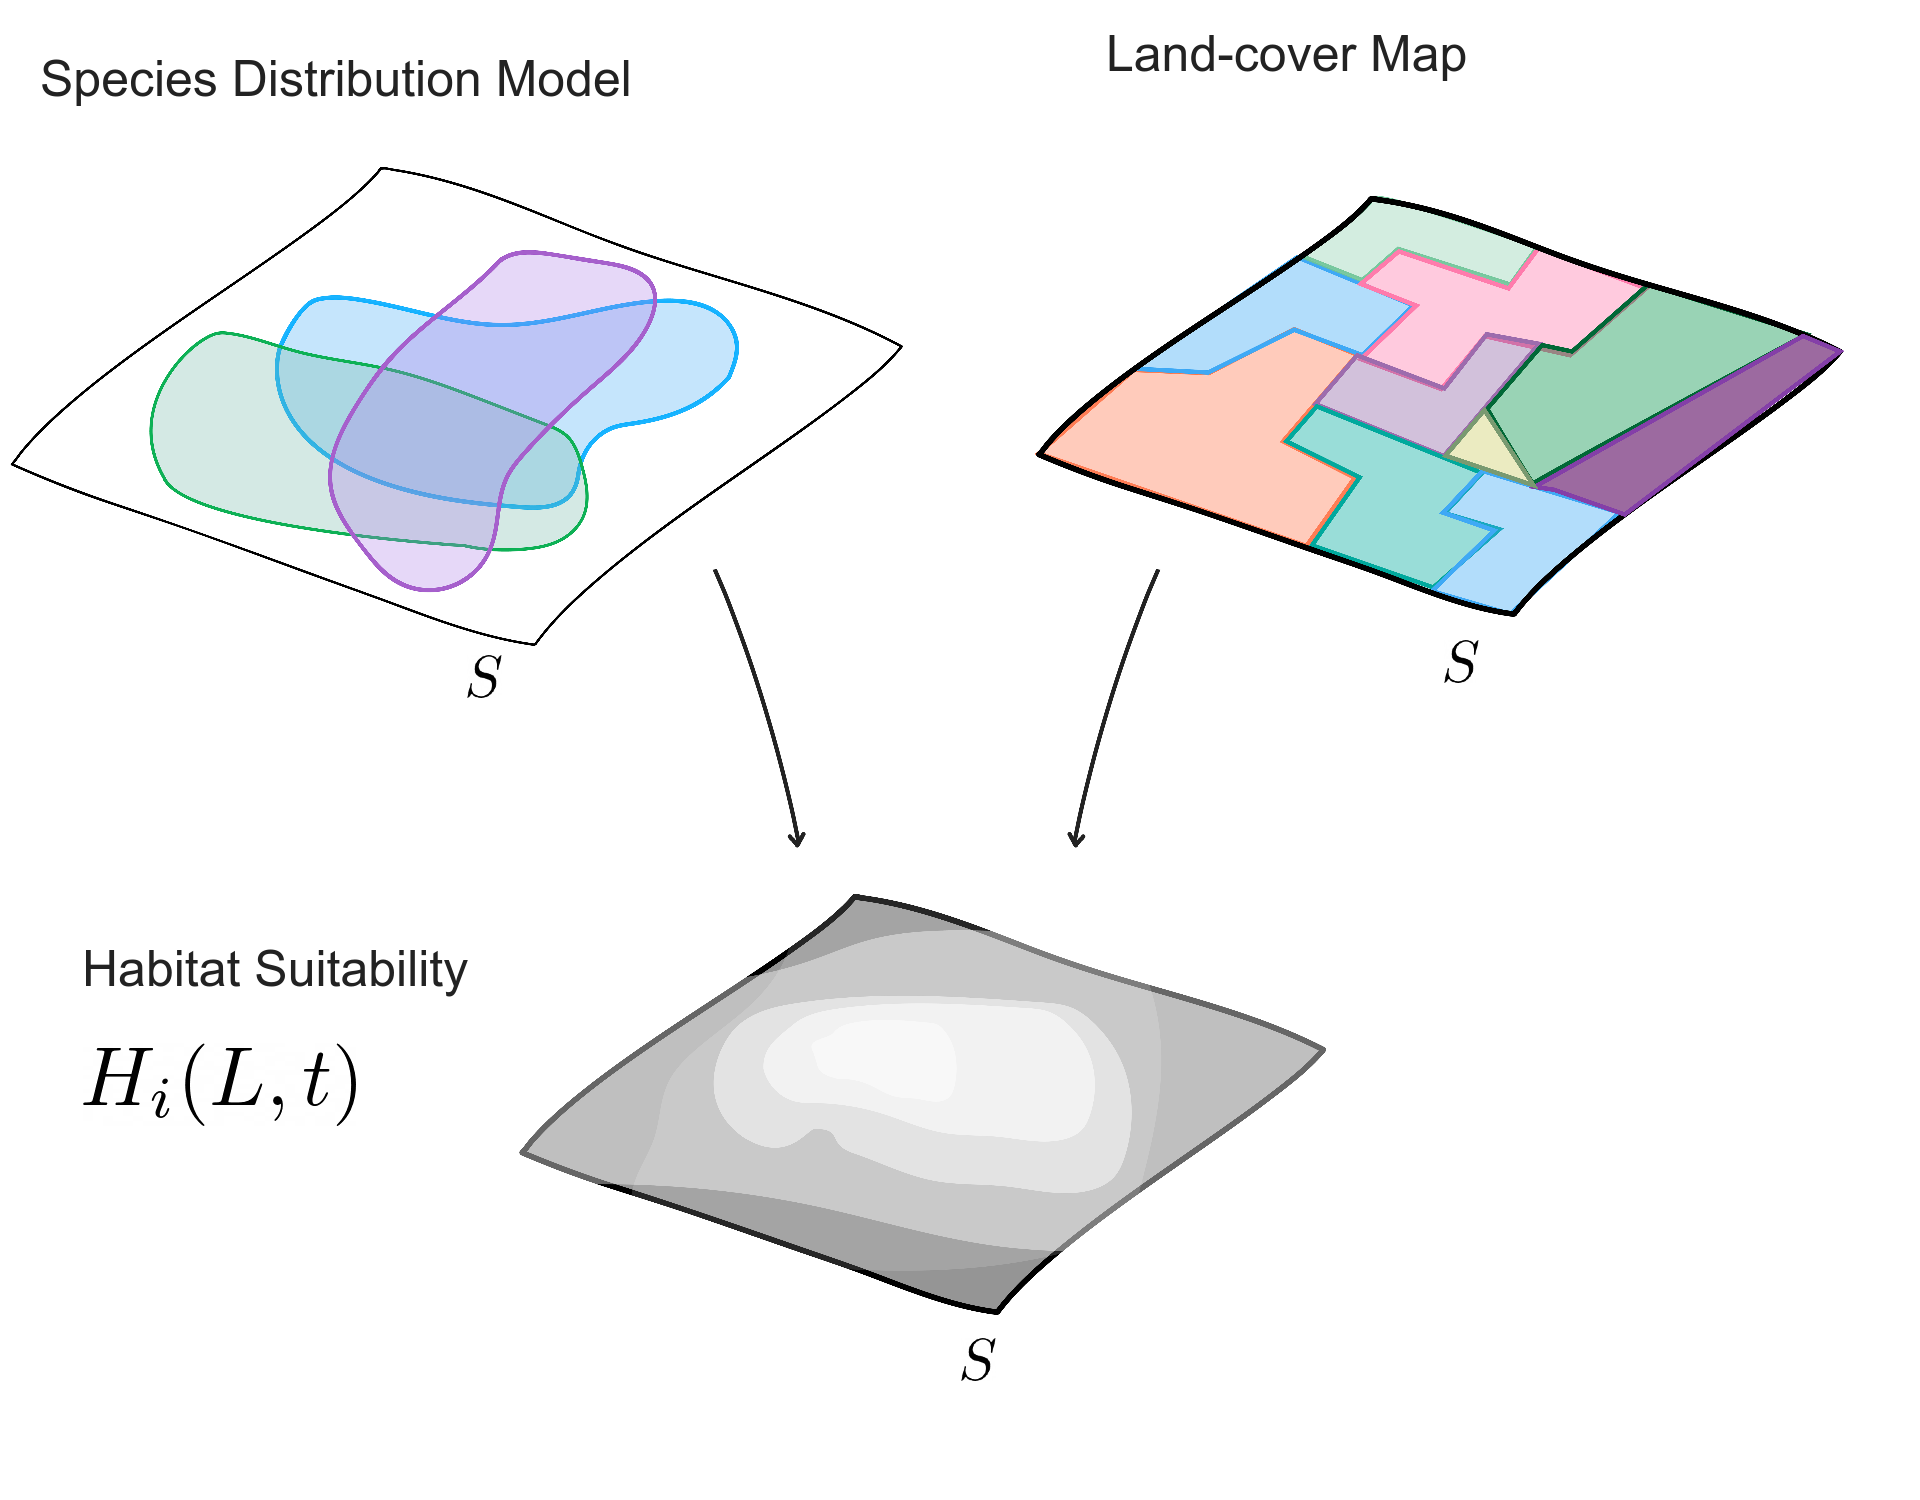
\includegraphics{/home/michael/prospectus/figures/habitat suitability w labels.png}
\caption{this is a caption}
\end{figure}

\begin{itemize}
\item
  spatial graph or a lattice \(L\) on a spatial domain \(S\)
\item
  abstraction of multiple environmental variables into a distribution of
  `habitat suitability',
\item
  however, this is a function of traits also \(H_i= f(T_i(L), E_i(L))\)
\item
  how does \(x_i\) affect \(x_j\)? we represent this as the dispersal
  potential \(\Phi = [\Phi_{ij}]\), where \(\Phi_{ij}\) is the
  probability that a unit biomass moves \(i \to j\) before reproducing.
\end{itemize}

\hypertarget{selection-model}{%
\subsection{3. Selection Model}\label{selection-model}}

Model of how that traits \(T_i\) and fitness \(\omega_i(L)\) change as a
function of \(H_i(x,t)\). One of the most well-studied problems in
evolutionary biology.

\[\frac{\partial T_i(x,t)}{\partial t} = f(T_i(x), H_i(x))\]

\hypertarget{measuring-metacommunity-structure}{%
\subsection{4. Measuring (Meta)community
Structure}\label{measuring-metacommunity-structure}}

\begin{itemize}
\tightlist
\item
  \(\hat{B}\) -- observed community at some time \(t\) and some location
  \(x_j\)
\item
  types of measures of network structure, \(C\)

  \begin{itemize}
  \tightlist
  \item
    \(C({\hat{B}(L_i)})\), singular.

    \begin{itemize}
    \tightlist
    \item
      a measure of \(\alpha\)-div at local community level
    \item
      most classic measures, Shannon entropy, etc.
    \end{itemize}
  \item
    \(C(\hat{B}(x_j), \hat{B}(x_k))\), measure of difference between two
    networks, \(\beta\)-diversity
  \item
    \(C(\hat{B})\) , measures of total structure across all locations
    (and times?), \(\gamma\)-diversity
  \end{itemize}
\end{itemize}

\pagebreak

\begin{figure}
\centering
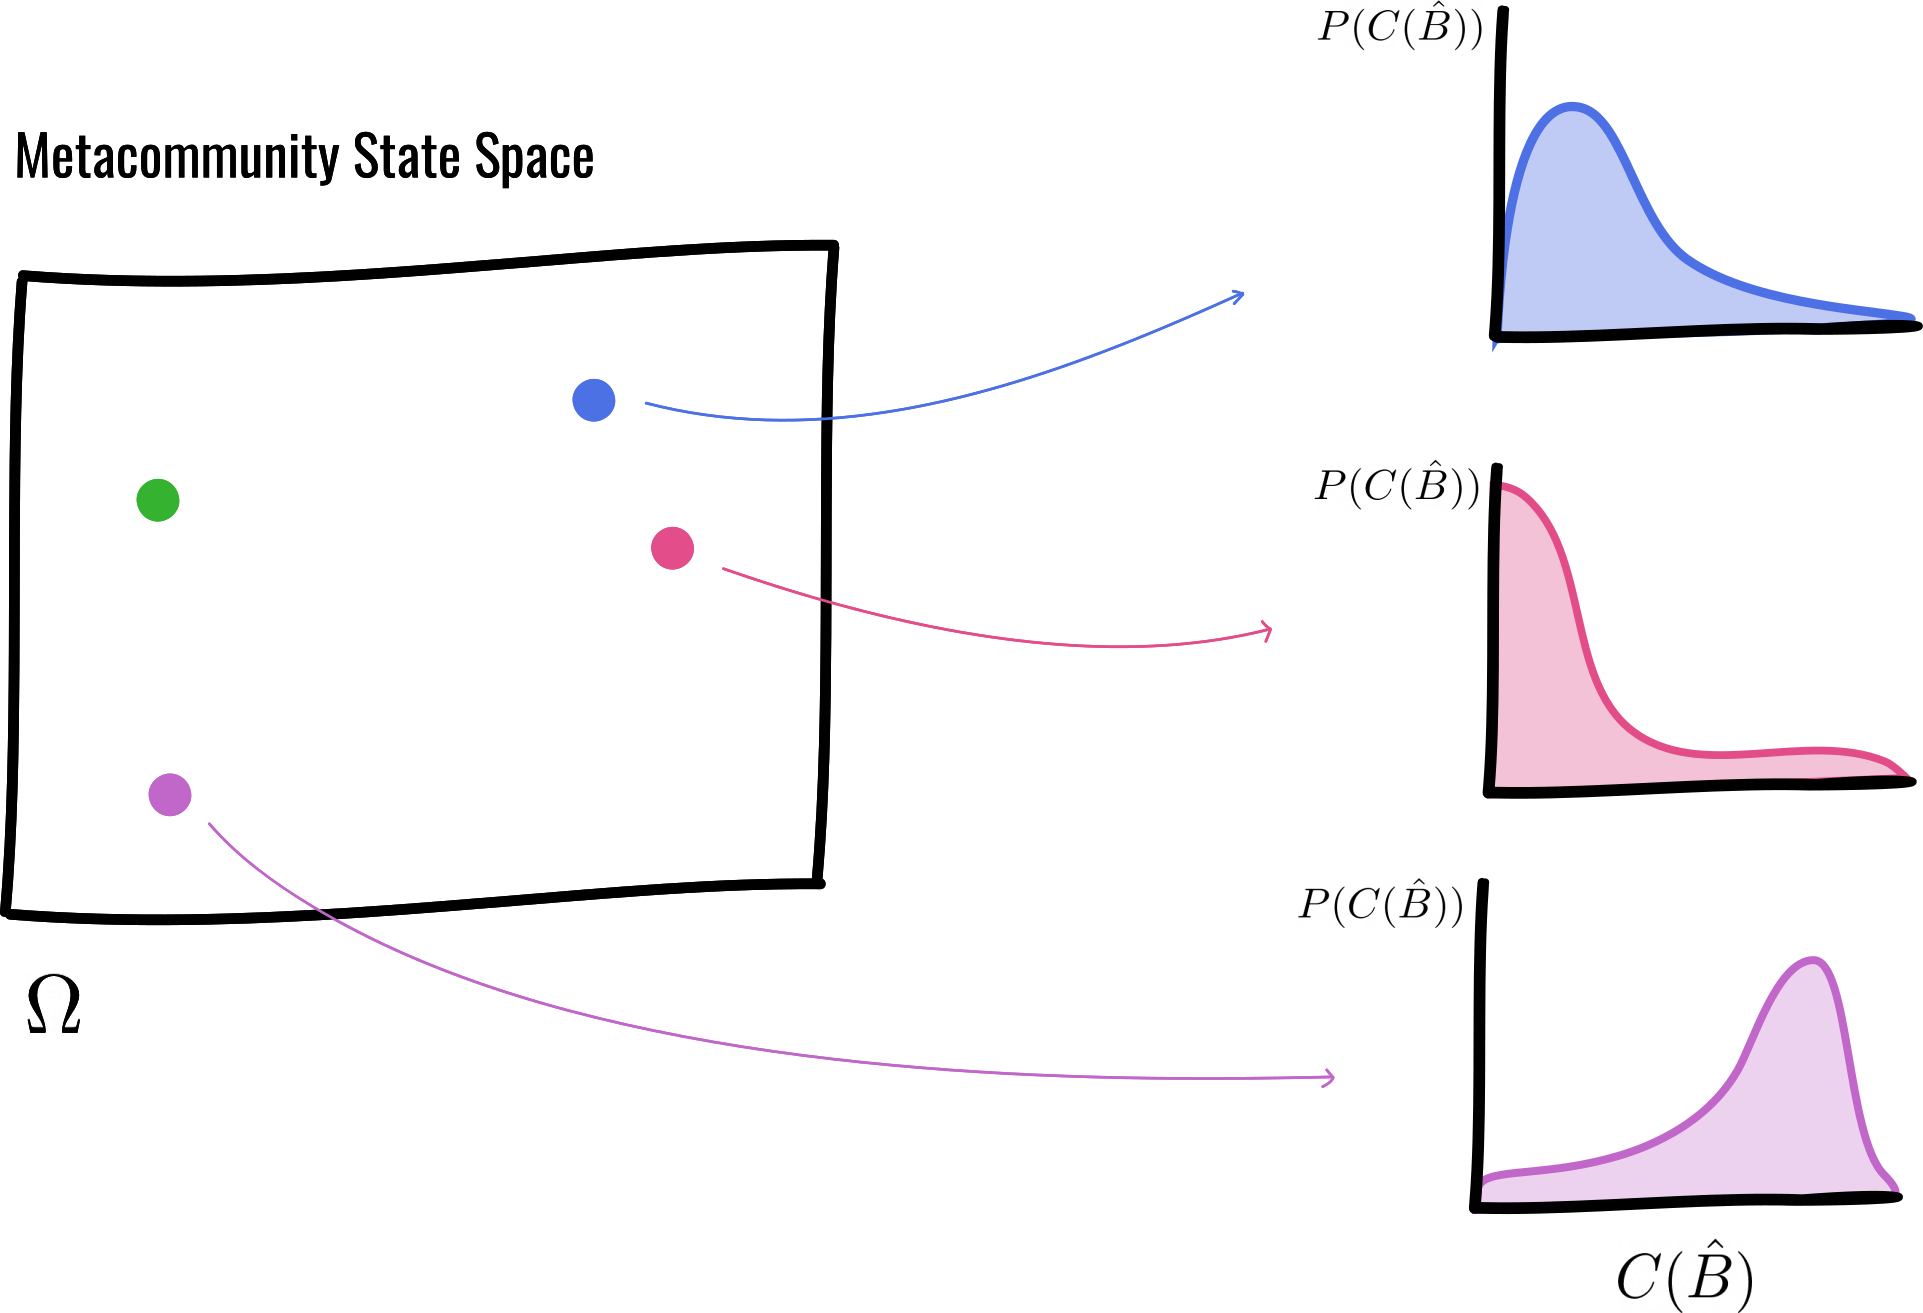
\includegraphics{/home/michael/prospectus/figures/metacomm_w_distributions.png}
\caption{this is a caption}
\end{figure}

Okay\ldots{}but how do you classify the `stability' of a non-equilibrium
system---

\begin{figure}
\centering
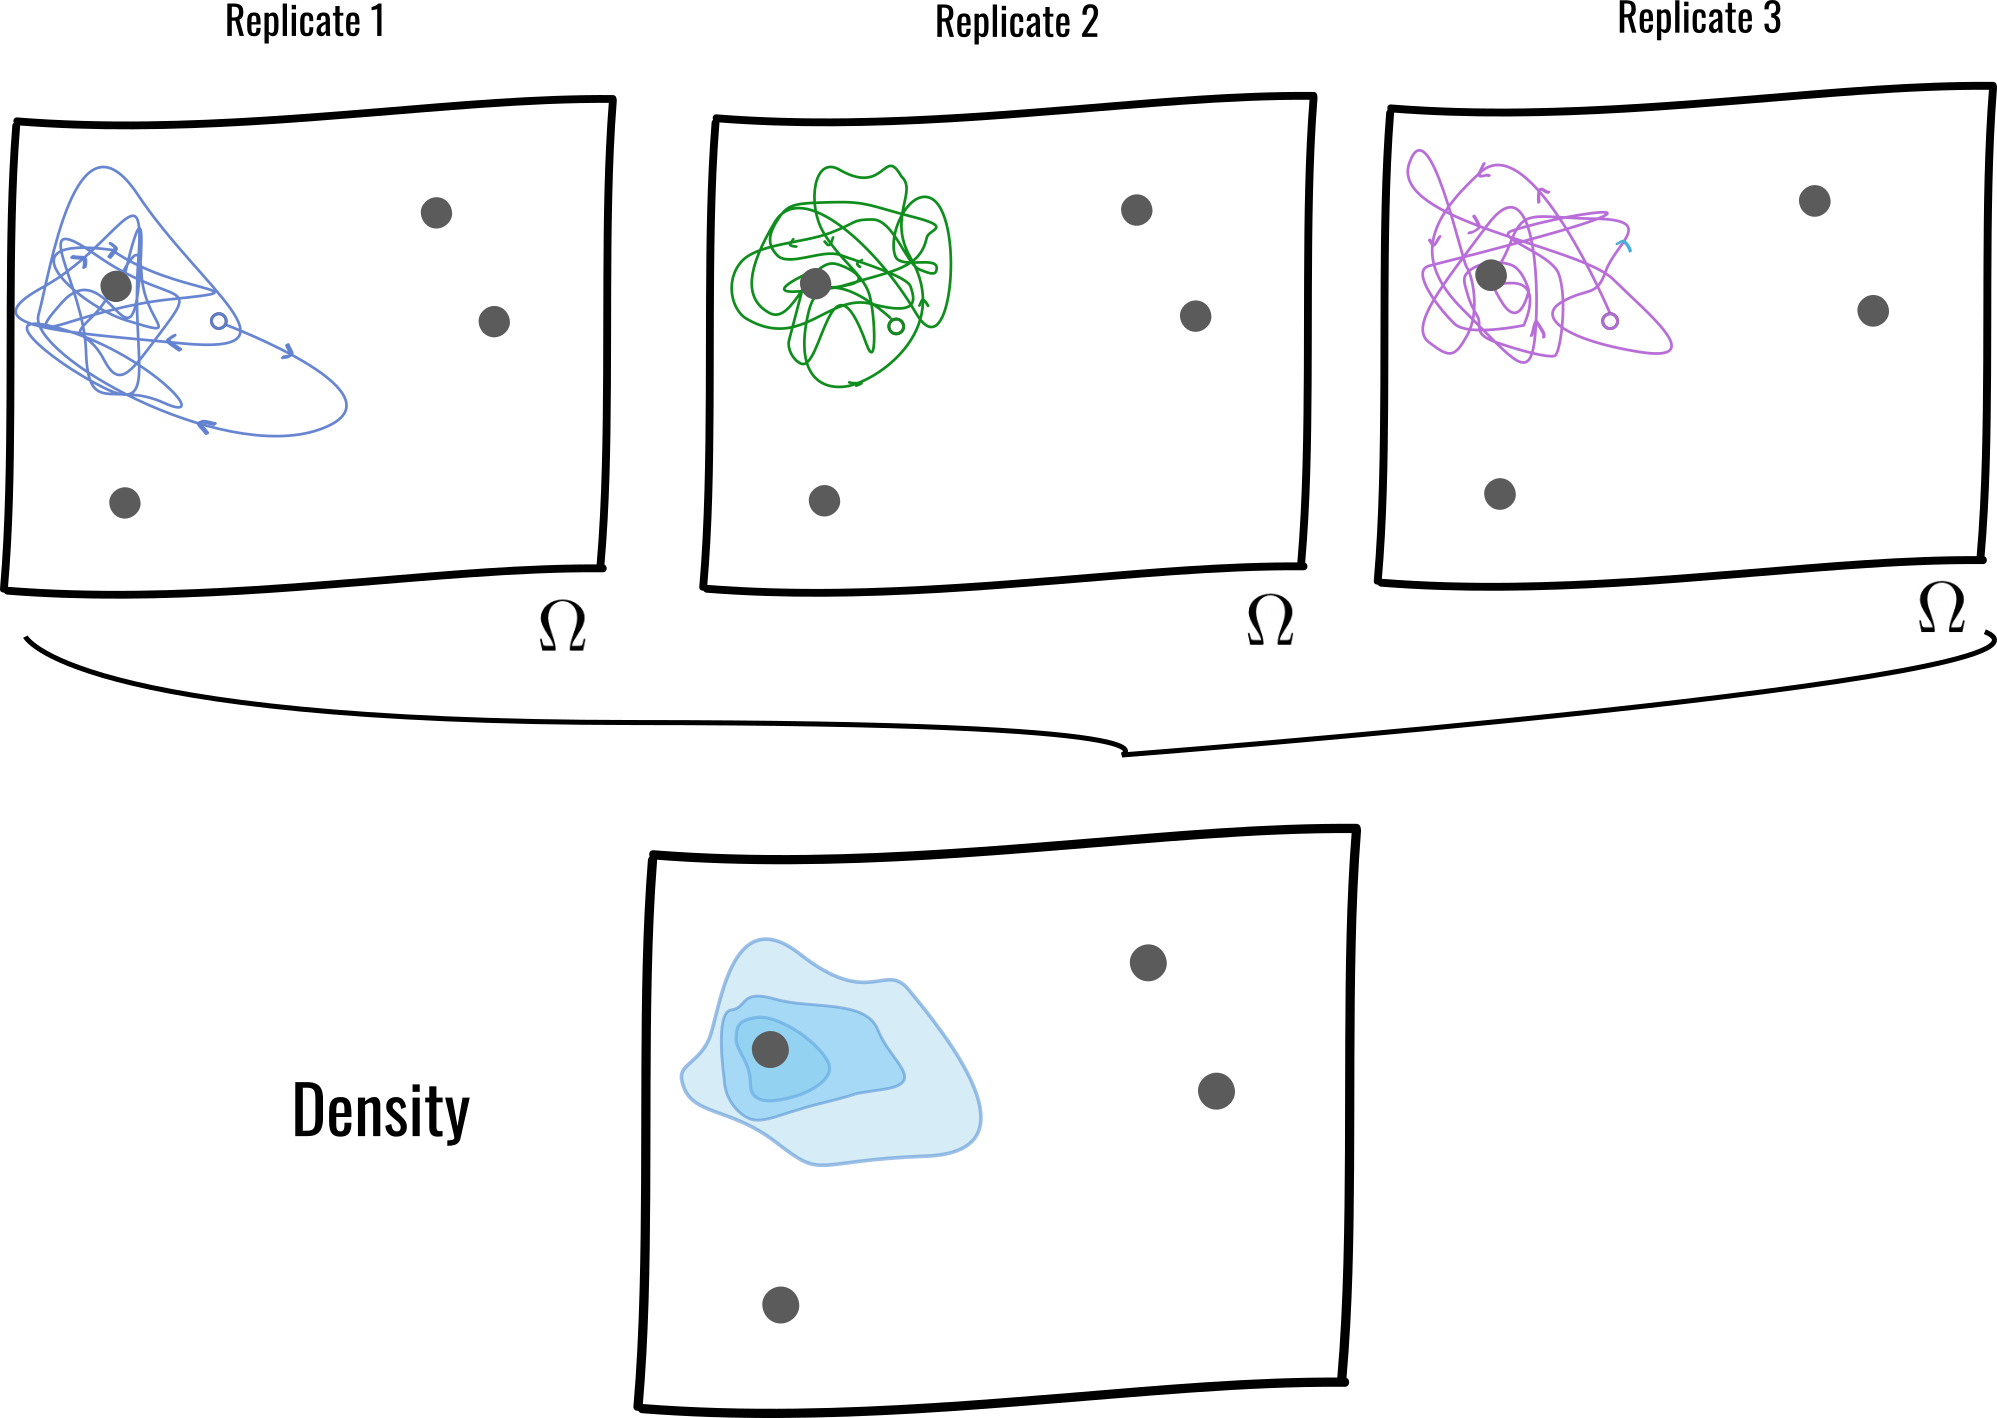
\includegraphics{/home/michael/prospectus/figures/density_plot.png}
\caption{this is a caption}
\end{figure}

\begin{figure}
\centering
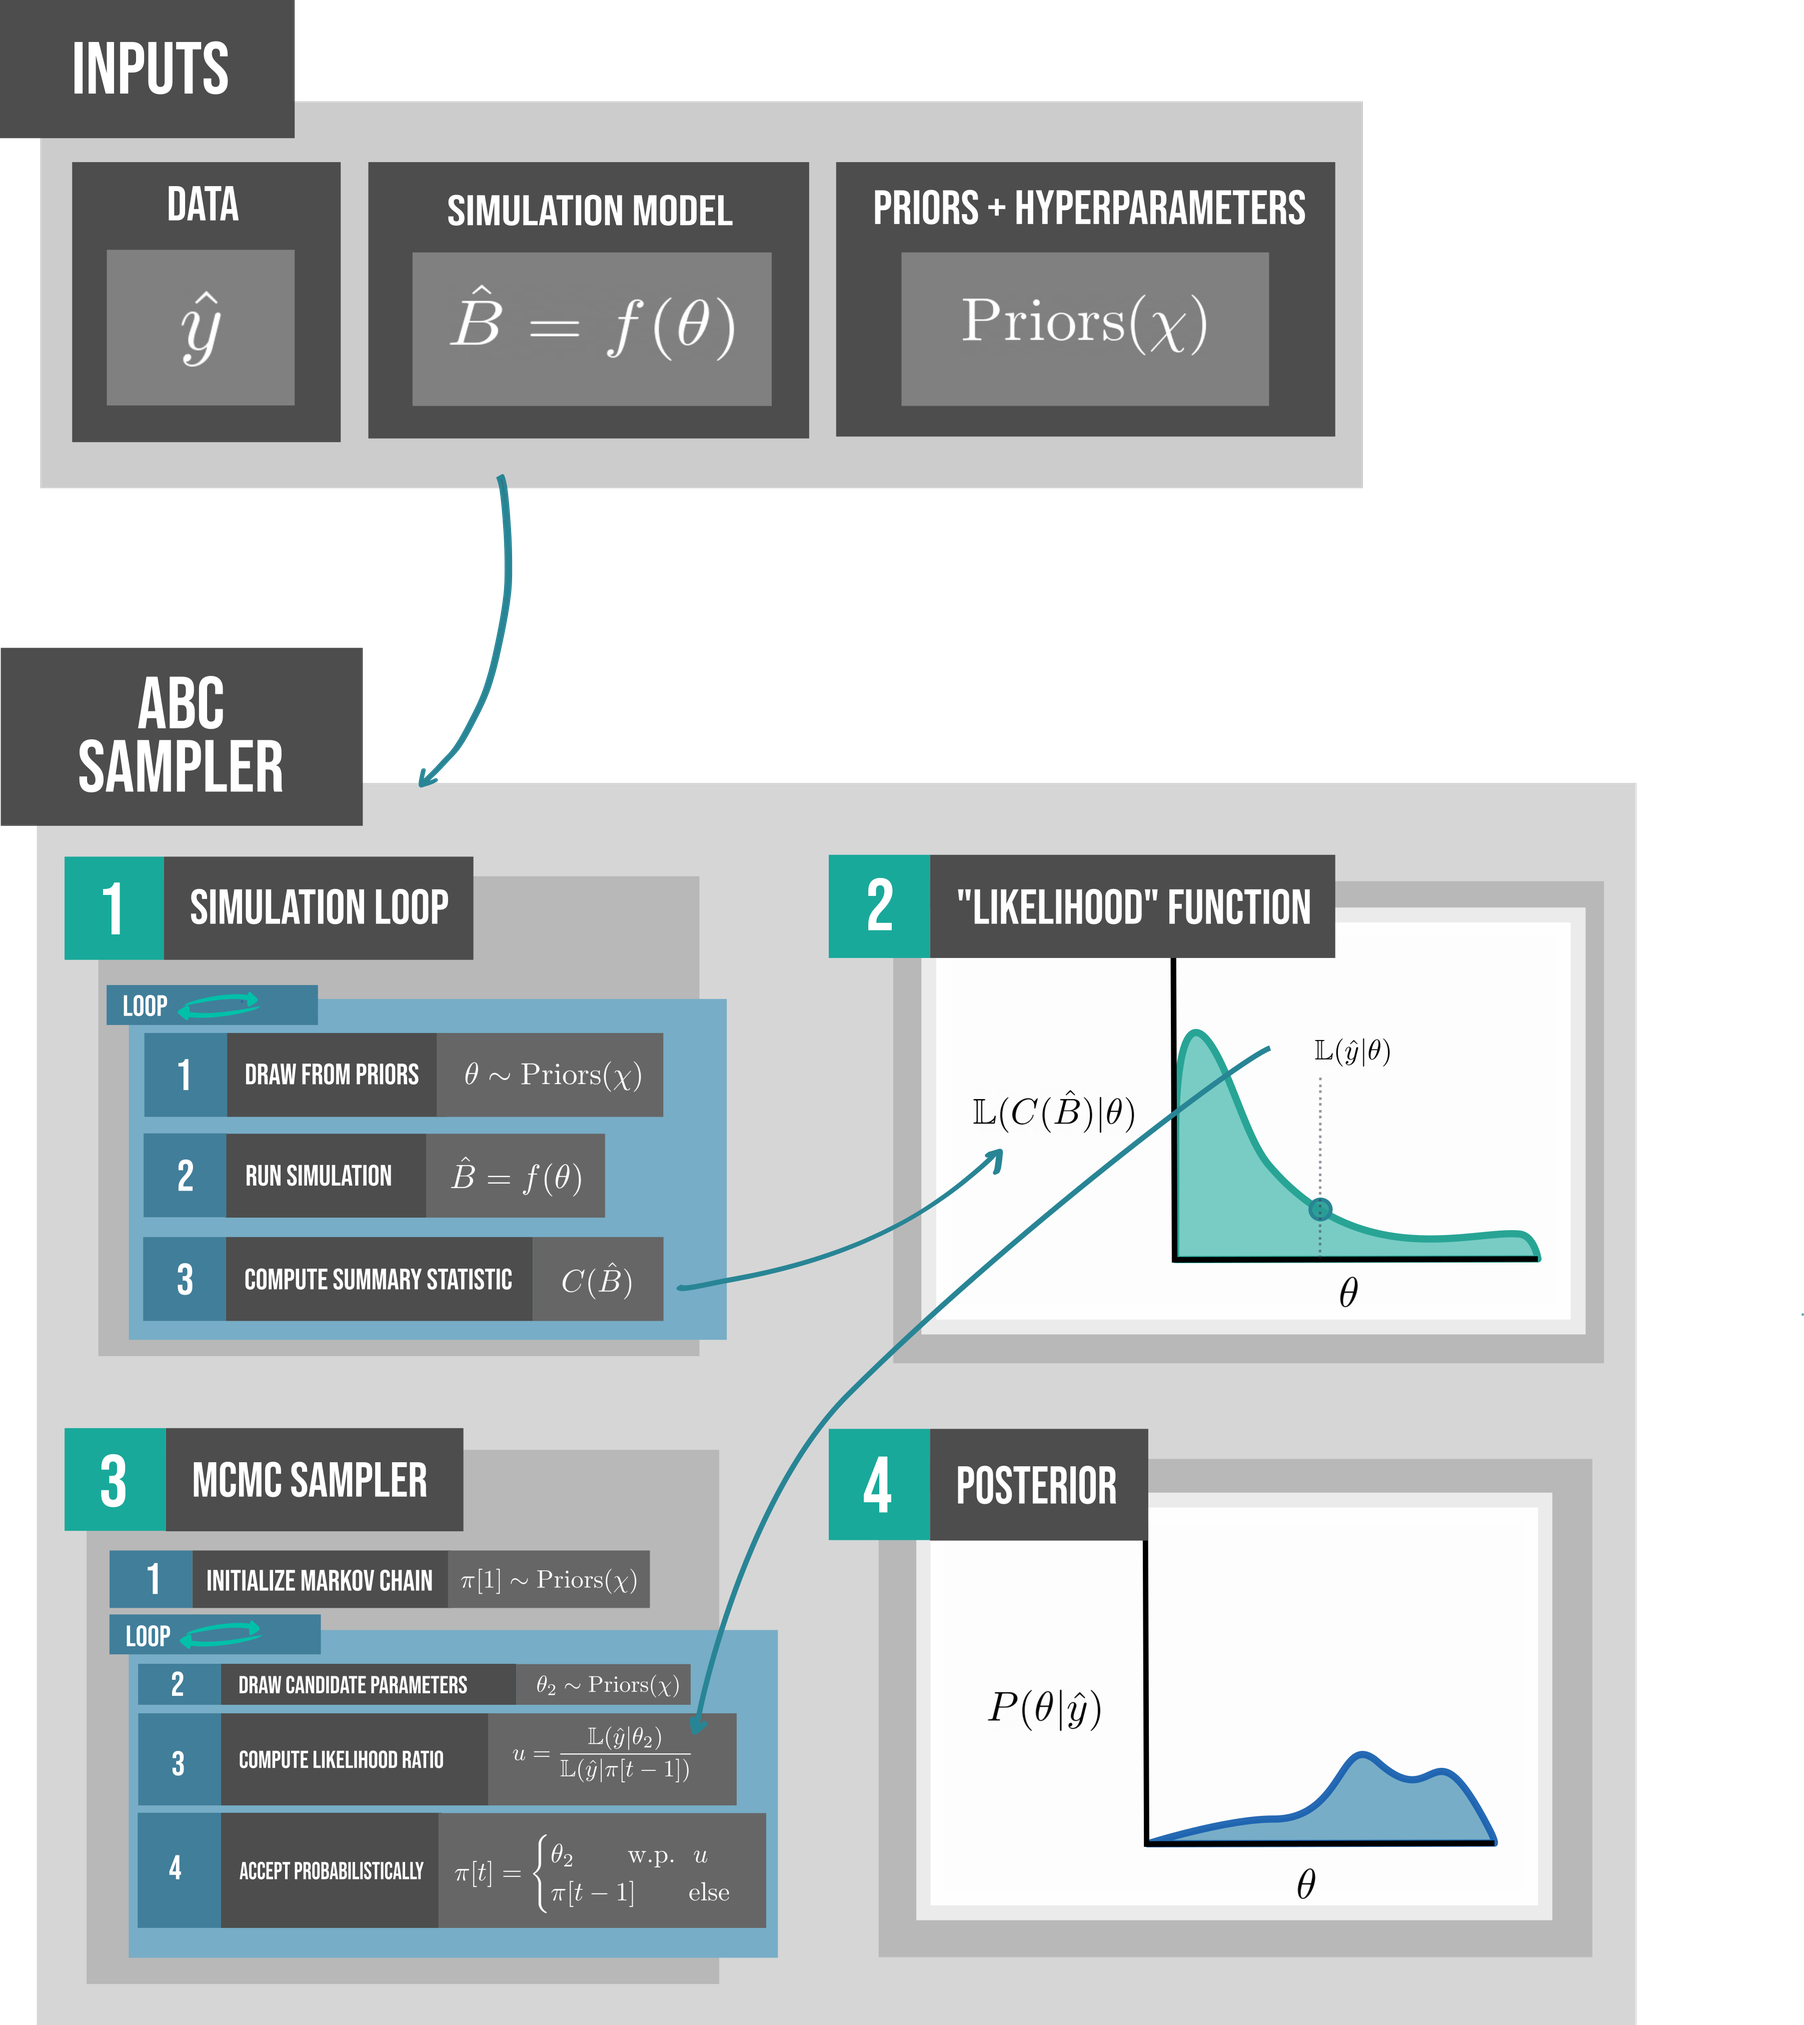
\includegraphics{/home/michael/prospectus/figures/abc_conceputal.png}
\caption{Conceptual overview of Approximate Bayesian Computation (ABC).
The version of an ABC Sampler presented here is methodologically the
simplest (and original) version, based on using a simulated likelihood
to run a rejection-based sampling MCMC algorithm. In panel 2
(top-right), to actually compute \(\mathbb{L}(\hat{y} | \theta)\) from
simulation outputs, traditionally one defineds an acceptance tolerance
\(\rho\), and accepts \(\hat{y} - y_{sim} < \rho\) . Alternatively, one
can run some regression on the on the simulation outcomes to get an
analytic approximation of \(\mathbb{L}(\hat{y} | \theta)\). More recent
improvements to ABC sampling deviate from simple rejection sampling
algorithms for efficiency, e.g.~doing rejection sampling whilst
composing the simulated likelihood to reduce the amount of time spent
running the simulation model in ``bad'' regions of parameter space---see
Adaptive Monte Carlo {[}@beaumont\_adaptive\_2009{]} and Sequential
Monte Carlo {[}@cite{]}.}
\end{figure}

\begin{figure}
\centering
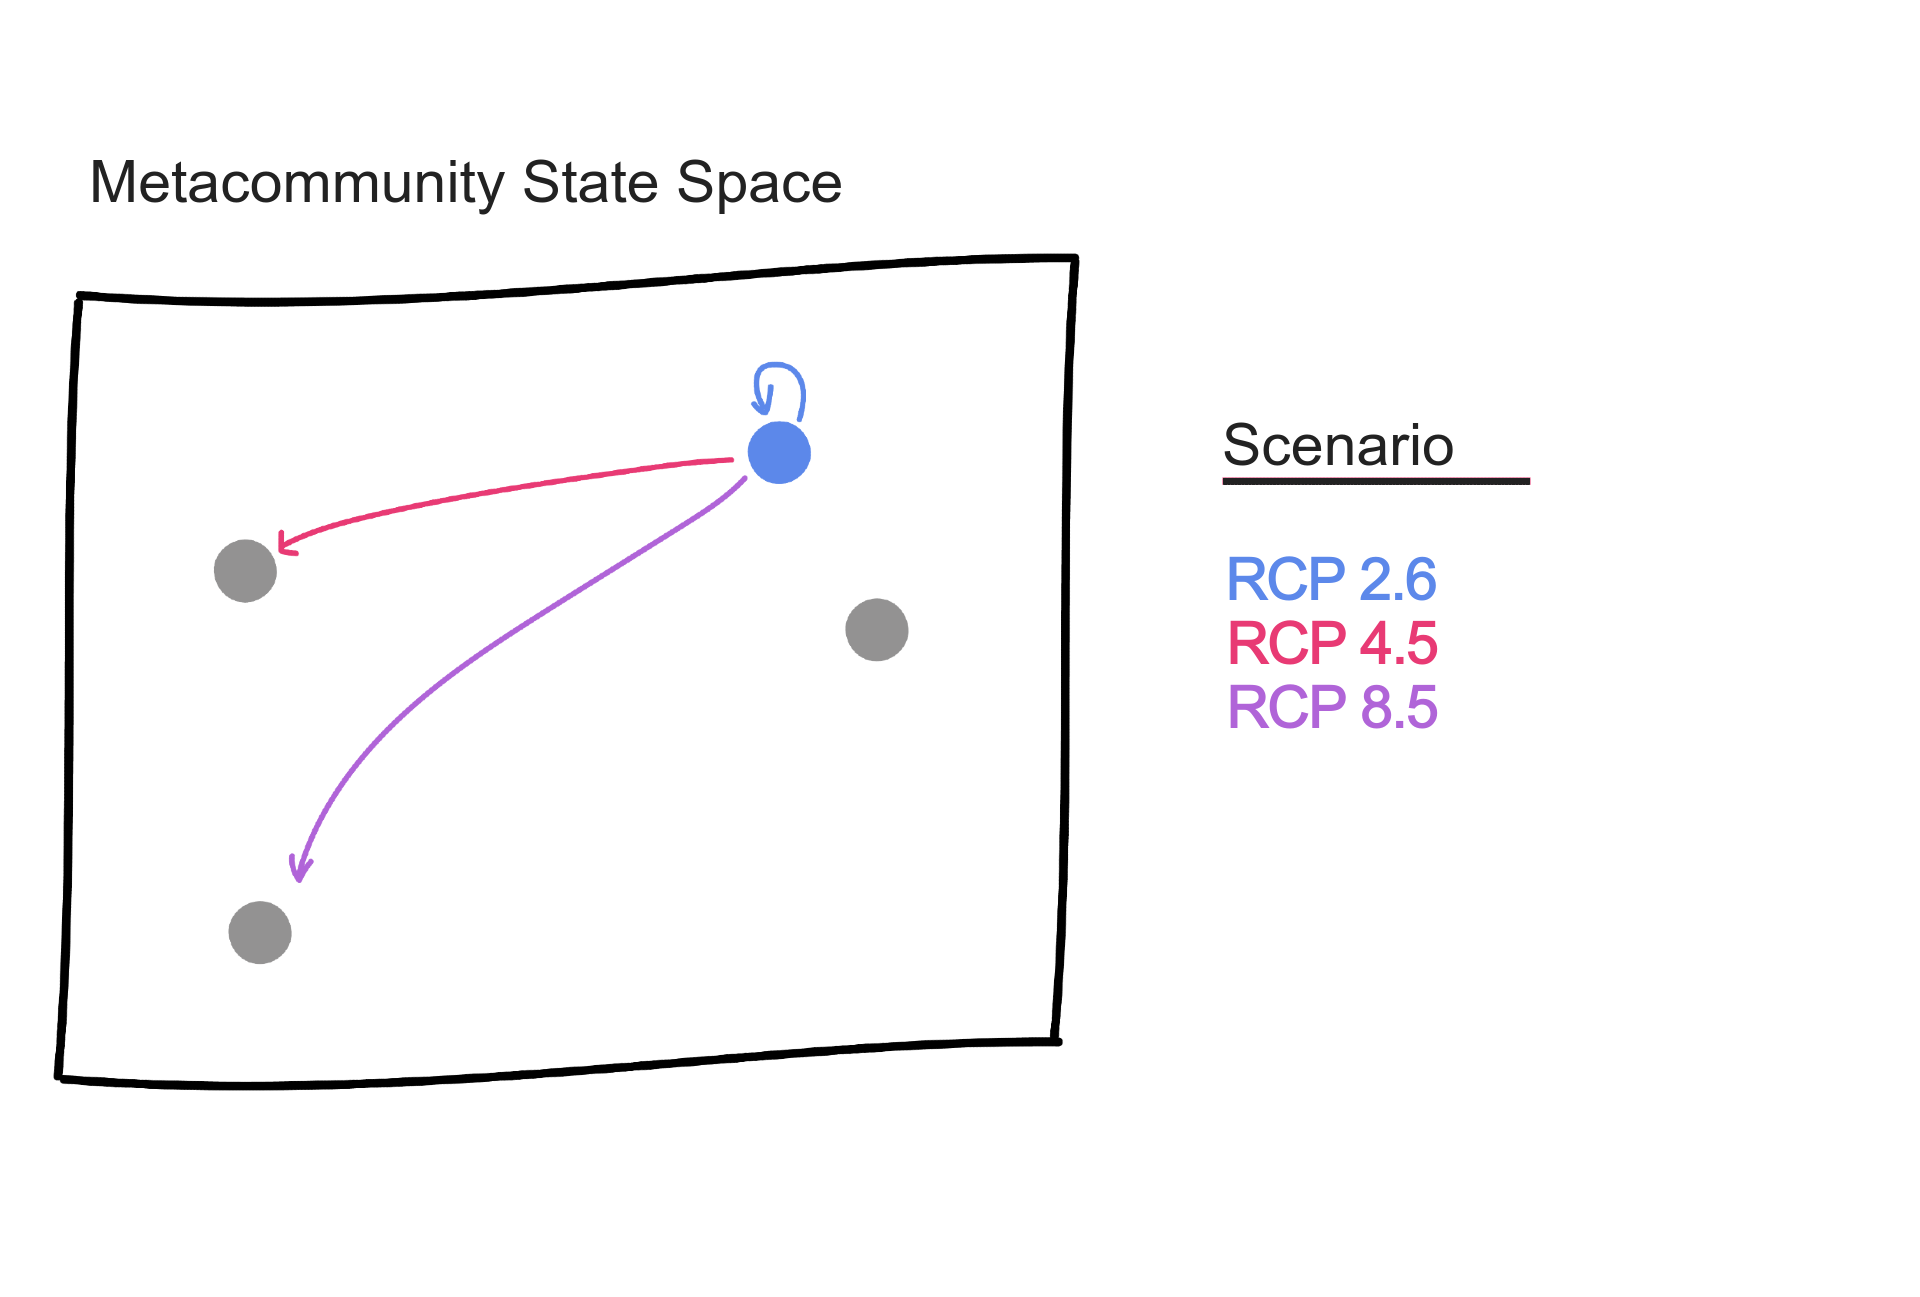
\includegraphics{/home/michael/prospectus/figures/different_scenarios.png}
\caption{This is the end goal of the dissertation. Build software that
can forecast the future state of metacommunity structure under proposed
forecasts of land-use/climate change, both for the data I apply it to,
but also be generalizable to different systems.}
\end{figure}

\begin{figure}
\centering
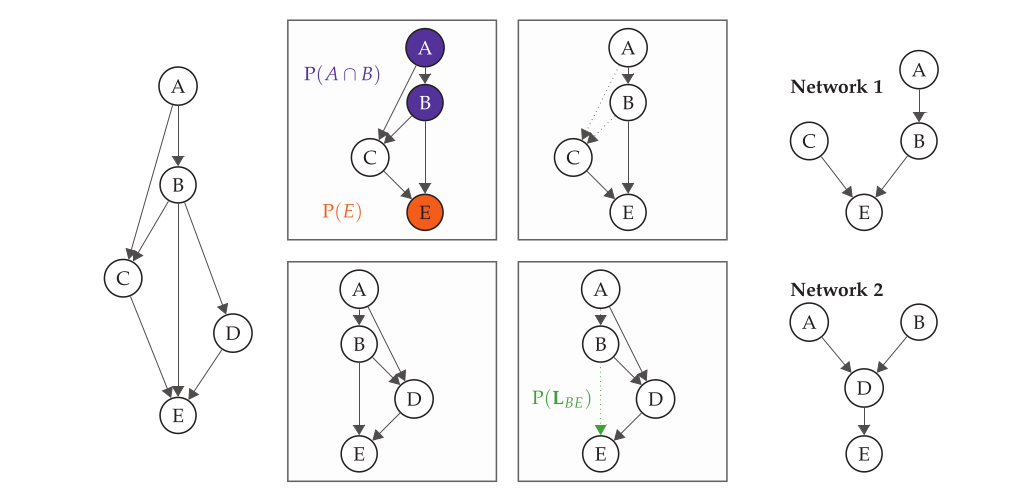
\includegraphics{/home/michael/prospectus/figures/poisot_metaweb_figure.png}
\caption{From Poisot et al.~(@poisot\_2015). Original Caption \emph{An
illustration of the metaweb concept. In its simplest form, a metaweb is
the list of all possible species and interactions between them for the
system being studied, at the regional level (far left side)Everything
that is ultimately observed in nature is a realisation of themetaweb
(far right side), i.e.~the resulting network after several sorting
processes have occurred (central panel). First, species and species
pairs have different probabilities to be observed (top panels). Second,
as a consequence of the mechanisms we outline in this paper, not
allinteractions have the same probability to occur at any given site
(bottom panels, see Box 1).}}
\end{figure}

\begin{figure}
\centering
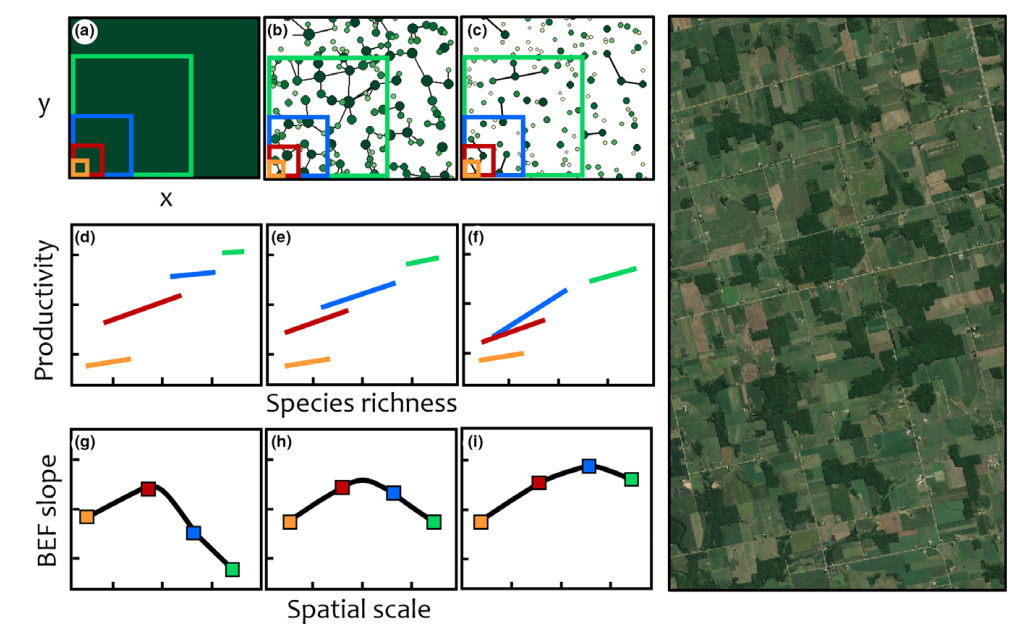
\includegraphics{/home/michael/prospectus/figures/gonzalez_ef_es.png}
\caption{From Gonzalez et al.~(@gonzalez\_bef\_2020). Original caption:
\emph{Figure 5 Right: Satellite image of an agricultural landscape with
remnant forest fragments. Left: Predictions for the change in BEF slope
as the scale of observation increases for three landscapes with varying
degrees of fragmentation (simulated data). Top row: Stylised landscapes
with different patterns of fragmentation of forest habitat (dark green)
and surrounding agriculture (white background): (a) homogeneous forest
(x = northing, y = easting), (b) fragments with varying diversity
(circle size) and productivity (circle greenness), with links indicating
connectivity by seed dispersal, (c) isolated fragments with lower
average diversity and productivity and fewer links. At each scale of
observation, denoted by the coloured sampling windows in (a--c), species
richness and productivity are measured at different locations across a
landscape by sliding the window. Middle row: Change in the linear
relationship between species richness and productivity at different
scales of observation for each landscape type (d--f). Each coloured line
is composed of measurements of species richness and productivity from
multiple windows at a given scale. Species richness and productivity
increases with the spatial scale of observation for all three landscape
types but the form of the BEF relationship varies. Bottom row: Change in
the BEF slope as a function of the scale of observation for each
landscape type (g--i). Each point corresponds to the value of the slope
of the line of same colour in the respective above figure. At a small
sampling scale (orange window in (a)) the BEF slope is low and similar
in all three landscape types (orange points in (g--i). At that scale,
species richness and productivity are small and not affected by
fragmentation (orange lines in (d--f)). At an intermediate sampling
scale (red window in (a)), the BEF slope increases in all three
landscape types. At that scale, sampling windows accounted for more
species richness and higher level of productivity leading to stronger
BEF effects. While fragmentation has reduced both biodiversity and
productivity (red lines in (d--f)), no notable impact on the BEF slope
is observed at this scale (red points (h--i)). At a large sampling scale
(blue) the BEF slope decreases in the homogeneous landscape (a, d, g)
since most species have already been sampled producing no additional
biodiversity effects on productivity. However, when fragments are
isolated (c), even if species richness and productivity are lower (f), a
wide range of species richness and productivity are sampled (blue line
in (f)) leading to an increase in BEF slope (blue point in (i)). The
effect of species turnover on the BEF slope is also observed, although
to a lesser degree, in the landscape with linked fragments (b, e, h)
since species turnover is reduced by the ability of species to disperse
across the landscape. At the largest sampling scale (green window in a)
the BEF slopes decrease in all three landscape types but at different
levels (green points in (g--i)). While productivity is higher at that
scale, species richness is similar in all sampling windows (green lines
in (d--f)).}}
\end{figure}

What does the software do?

\begin{itemize}
\tightlist
\item
  software that is modular and can be fit to data in real systems in
  multiple ways

  \begin{itemize}
  \tightlist
  \item
    you can provide, \(A\), or \(S\), different versions of a selection
    function \(S\)
  \end{itemize}
\item
  simulation can be used to explore the properties of complex systems on
  scales larger than can be observed.
\item
  using approx. Bayes comp. to fit the results of complex simulation
  models to data
\item
  identify fixed points for a given food web topology, and forecast its
  behavior under hypothetical environment/land use scenarios
\end{itemize}

Major Questions

\begin{itemize}
\tightlist
\item
  differentiating niche vs neutral processes in metacommunity assembly,
  across spatial scale
\item
  critical transitions in community structure

  \begin{itemize}
  \tightlist
  \item
    when we change strength of environmental factors in shifting
    survivability/traits
  \item
    when we change dispersal (connectivity, etc)Major Questions
  \end{itemize}
\end{itemize}

What can we use models to infer?

Niche vs.~Neutral

environmental conditions and their relation to ranges and interactions

dispersal and neutral colonization/extinction

Poisot 2014 model of interaction networks. Relates to the properties we
can measure.

\hypertarget{dissertation-outline}{%
\section{Dissertation Outline}\label{dissertation-outline}}

\hypertarget{chapter-one}{%
\subsection{Chapter One}\label{chapter-one}}

\begin{itemize}
\item
  Introduction and Literature Review
\item
  Looks a lot like this document but with a more in-depth review
\end{itemize}

\hypertarget{chapter-two}{%
\subsection{Chapter Two}\label{chapter-two}}

\begin{itemize}
\tightlist
\item
  The model software paper
\end{itemize}

\hypertarget{chapter-three}{%
\subsection{Chapter Three}\label{chapter-three}}

\begin{itemize}
\tightlist
\item
  At what spatial scales do processes shift from being neutral to niche?
\end{itemize}

\hypertarget{chapter-four}{%
\subsection{Chapter Four}\label{chapter-four}}

\begin{itemize}
\tightlist
\item
  Applying model to specifics system for forecasting under land use and
  climate change
\end{itemize}

\hypertarget{chapter-five}{%
\subsection{Chapter Five}\label{chapter-five}}

\begin{itemize}
\tightlist
\item
  Applying model to inference in large datasets
\end{itemize}

\hypertarget{table-of-symbols}{%
\section{Table of Symbols}\label{table-of-symbols}}

\begin{longtable}[]{@{}ccl@{}}
\toprule
\begin{minipage}[b]{0.25\columnwidth}\centering
Name\strut
\end{minipage} & \begin{minipage}[b]{0.23\columnwidth}\centering
Symbol\strut
\end{minipage} & \begin{minipage}[b]{0.42\columnwidth}\raggedright
Meaning\strut
\end{minipage}\tabularnewline
\midrule
\endhead
\begin{minipage}[t]{0.25\columnwidth}\centering
Concept Space\strut
\end{minipage} & \begin{minipage}[t]{0.23\columnwidth}\centering
\(A\)\strut
\end{minipage} & \begin{minipage}[t]{0.42\columnwidth}\raggedright
the set of conceptual objects designed to represent scientific one could
define in a scientific model \(f\)\strut
\end{minipage}\tabularnewline
\begin{minipage}[t]{0.25\columnwidth}\centering
State Space\strut
\end{minipage} & \begin{minipage}[t]{0.23\columnwidth}\centering
\(\Omega\)\strut
\end{minipage} & \begin{minipage}[t]{0.42\columnwidth}\raggedright
the set of possible states a given system (respresented using a concept
set \(A\)) could exist in at any given time. \(\Omega\) can be thought
of as the span of \(O(A)\).\strut
\end{minipage}\tabularnewline
\begin{minipage}[t]{0.25\columnwidth}\centering
Observation Function\strut
\end{minipage} & \begin{minipage}[t]{0.23\columnwidth}\centering
\(O\)\strut
\end{minipage} & \begin{minipage}[t]{0.42\columnwidth}\raggedright
a function which maps conceptual objects in our models to observations,
which typically (but not necessarily) take the form of real
numbers\strut
\end{minipage}\tabularnewline
\begin{minipage}[t]{0.25\columnwidth}\centering
Scientific Model\strut
\end{minipage} & \begin{minipage}[t]{0.23\columnwidth}\centering
\(f\)\strut
\end{minipage} & \begin{minipage}[t]{0.42\columnwidth}\raggedright
the set of conceptual objects designed to represent scientific one could
define in a scientific model\strut
\end{minipage}\tabularnewline
\begin{minipage}[t]{0.25\columnwidth}\centering
Parameter Space\strut
\end{minipage} & \begin{minipage}[t]{0.23\columnwidth}\centering
\(\Theta\)\strut
\end{minipage} & \begin{minipage}[t]{0.42\columnwidth}\raggedright
the set of possible values the parameters \(\theta\) of a model \(f\)
could have\strut
\end{minipage}\tabularnewline
\begin{minipage}[t]{0.25\columnwidth}\centering
Dispersal Potential\strut
\end{minipage} & \begin{minipage}[t]{0.23\columnwidth}\centering
\(\Phi_{ij}\)\strut
\end{minipage} & \begin{minipage}[t]{0.42\columnwidth}\raggedright
the probability that an individual born in \(i\) dies in \(j\)\strut
\end{minipage}\tabularnewline
\begin{minipage}[t]{0.25\columnwidth}\centering
Spatial Domain\strut
\end{minipage} & \begin{minipage}[t]{0.23\columnwidth}\centering
\(S\)\strut
\end{minipage} & \begin{minipage}[t]{0.42\columnwidth}\raggedright
the space in which spatial locations \(L\) are represented as
coordinates\strut
\end{minipage}\tabularnewline
\begin{minipage}[t]{0.25\columnwidth}\centering
Spatial Locations\strut
\end{minipage} & \begin{minipage}[t]{0.23\columnwidth}\centering
\(L\)\strut
\end{minipage} & \begin{minipage}[t]{0.42\columnwidth}\raggedright
the set of locations \(L_i \in S\) , each with a coordinate\strut
\end{minipage}\tabularnewline
\begin{minipage}[t]{0.25\columnwidth}\centering
Probability Space\strut
\end{minipage} & \begin{minipage}[t]{0.23\columnwidth}\centering
\(\mathbb{P}\)\strut
\end{minipage} & \begin{minipage}[t]{0.42\columnwidth}\raggedright
the combined set of a state space \(\Omega\), a \(\sigma\)-algebra of
events within the set the states, \({F} \in \Omega\) , and a probability
measure \(P\) which maps any \({F} \in \Omega\) to a number between
\(0\) and \(1\)\strut
\end{minipage}\tabularnewline
\begin{minipage}[t]{0.25\columnwidth}\centering
Trait Distribution\strut
\end{minipage} & \begin{minipage}[t]{0.23\columnwidth}\centering
\(T_i(x,t)\)\strut
\end{minipage} & \begin{minipage}[t]{0.42\columnwidth}\raggedright
the distribution of traits at population \(i\) as a function of time.
here \(T_i(x,t)\) is a probability density function over \(x \in [0,1]\)
for any given population \(i\).\strut
\end{minipage}\tabularnewline
\begin{minipage}[t]{0.25\columnwidth}\centering
Bioenergetic Model\strut
\end{minipage} & \begin{minipage}[t]{0.23\columnwidth}\centering
\[\frac{\partial B}{\partial t}\]\strut
\end{minipage} & \begin{minipage}[t]{0.42\columnwidth}\raggedright
describes the flow of energy stored as biomass on a food web\strut
\end{minipage}\tabularnewline
\begin{minipage}[t]{0.25\columnwidth}\centering
Likelihood Function\strut
\end{minipage} & \begin{minipage}[t]{0.23\columnwidth}\centering
\(\mathbb{L}(\hat{x} | \theta)\)\strut
\end{minipage} & \begin{minipage}[t]{0.42\columnwidth}\raggedright
a mapping from a combination of state and parameter values to a
probability of that combination occurring under some model \(f\)\strut
\end{minipage}\tabularnewline
\begin{minipage}[t]{0.25\columnwidth}\centering
Posterior Distribution\strut
\end{minipage} & \begin{minipage}[t]{0.23\columnwidth}\centering
\(P(\theta | \hat{x})\)\strut
\end{minipage} & \begin{minipage}[t]{0.42\columnwidth}\raggedright
the probability distribution of a parameter \(\theta\) given some data
\(\hat{x}\) and a prior \(P(\theta)\)\strut
\end{minipage}\tabularnewline
\begin{minipage}[t]{0.25\columnwidth}\centering
Prior Distribution\strut
\end{minipage} & \begin{minipage}[t]{0.23\columnwidth}\centering
\(P(\theta)\)\strut
\end{minipage} & \begin{minipage}[t]{0.42\columnwidth}\raggedright
an a priori estimate of the distribution of a parameter \(\theta\)\strut
\end{minipage}\tabularnewline
\begin{minipage}[t]{0.25\columnwidth}\centering
Parameters\strut
\end{minipage} & \begin{minipage}[t]{0.23\columnwidth}\centering
\(\theta\)\strut
\end{minipage} & \begin{minipage}[t]{0.42\columnwidth}\raggedright
the parameters of any given model \(f\)\strut
\end{minipage}\tabularnewline
\begin{minipage}[t]{0.25\columnwidth}\centering
Metaweb\strut
\end{minipage} & \begin{minipage}[t]{0.23\columnwidth}\centering
\(M\)\strut
\end{minipage} & \begin{minipage}[t]{0.42\columnwidth}\raggedright
a network of possible interactions between species, typically
represented as an adjacency matrix\strut
\end{minipage}\tabularnewline
\begin{minipage}[t]{0.25\columnwidth}\centering
\strut
\end{minipage} & \begin{minipage}[t]{0.23\columnwidth}\centering
\strut
\end{minipage} & \begin{minipage}[t]{0.42\columnwidth}\raggedright
\strut
\end{minipage}\tabularnewline
\begin{minipage}[t]{0.25\columnwidth}\centering
\strut
\end{minipage} & \begin{minipage}[t]{0.23\columnwidth}\centering
\strut
\end{minipage} & \begin{minipage}[t]{0.42\columnwidth}\raggedright
\strut
\end{minipage}\tabularnewline
\begin{minipage}[t]{0.25\columnwidth}\centering
Biomass Vector\strut
\end{minipage} & \begin{minipage}[t]{0.23\columnwidth}\centering
\(\vec{B}\)\strut
\end{minipage} & \begin{minipage}[t]{0.42\columnwidth}\raggedright
\strut
\end{minipage}\tabularnewline
\begin{minipage}[t]{0.25\columnwidth}\centering
Biomass vector observation\strut
\end{minipage} & \begin{minipage}[t]{0.23\columnwidth}\centering
\(\hat{B}\)\strut
\end{minipage} & \begin{minipage}[t]{0.42\columnwidth}\raggedright
\strut
\end{minipage}\tabularnewline
\begin{minipage}[t]{0.25\columnwidth}\centering
Community Structure Summary Function\strut
\end{minipage} & \begin{minipage}[t]{0.23\columnwidth}\centering
\(C(\hat{B})\)\strut
\end{minipage} & \begin{minipage}[t]{0.42\columnwidth}\raggedright
\strut
\end{minipage}\tabularnewline
\begin{minipage}[t]{0.25\columnwidth}\centering
Habitat Suitability Function\strut
\end{minipage} & \begin{minipage}[t]{0.23\columnwidth}\centering
\(H_i(L_j,t)\)\strut
\end{minipage} & \begin{minipage}[t]{0.42\columnwidth}\raggedright
the habitat suitability of species \(i\) and locations \(L_j\) at time
\(t\)\strut
\end{minipage}\tabularnewline
\begin{minipage}[t]{0.25\columnwidth}\centering
Set of species\strut
\end{minipage} & \begin{minipage}[t]{0.23\columnwidth}\centering
\(\mathbb{S}\)\strut
\end{minipage} & \begin{minipage}[t]{0.42\columnwidth}\raggedright
\strut
\end{minipage}\tabularnewline
\begin{minipage}[t]{0.25\columnwidth}\centering
Time domain\strut
\end{minipage} & \begin{minipage}[t]{0.23\columnwidth}\centering
\(\tau\)\strut
\end{minipage} & \begin{minipage}[t]{0.42\columnwidth}\raggedright
\strut
\end{minipage}\tabularnewline
\begin{minipage}[t]{0.25\columnwidth}\centering
\strut
\end{minipage} & \begin{minipage}[t]{0.23\columnwidth}\centering
\strut
\end{minipage} & \begin{minipage}[t]{0.42\columnwidth}\raggedright
\strut
\end{minipage}\tabularnewline
\bottomrule
\end{longtable}

\pagebreak

\hypertarget{references}{%
\section{References}\label{references}}
